\documentclass[smallcondensed]{svjour3}
\usepackage{amsmath}
\usepackage{multirow}
\usepackage[usenames, dvipsnames]{color}
\usepackage{colortbl}

\usepackage{balance}
\usepackage{array}
\usepackage{times}
\usepackage{tabularx}


\usepackage{picture}
\usepackage{wrapfig}
\usepackage{algorithm}
\usepackage{graphicx}
\usepackage{algorithmicx}
\usepackage{algpseudocode}
\renewcommand{\algorithmicrequire}{\textbf{Input:}}
\renewcommand{\algorithmicensure}{\textbf{Output:}} 
\newcommand{\lucas}[1]{\textcolor{red}{LUCAS: #1}} 
\newcommand{\tim}[1]{\textcolor{Red}{TIM: #1}}
\newcommand{\bill}[1]{\textcolor{blue}{BILL: #1}} 
\newcommand{\carter}[1]{\textcolor{cyan}{CARTER: #1}} 
\newcommand{\sei}[1]{\textcolor{RedViolet}{BILL/FORREST: #1}} 
\newcommand{\todo}[1]{\textcolor{Maroon}{TODO: #1}} 
%\newenvironment{changed}{\par}{\par}

%timm tricks
\newcommand{\bi}{\begin{itemize}}%[leftmargin=0.4cm]}
\newcommand{\ei}{\end{itemize}}
\newcommand{\be}{\begin{enumerate}}
\newcommand{\ee}{\end{enumerate}}
\newcommand{\tion}[1]{\S\ref{sect:#1}}
\newcommand{\fig}[1]{Figure~\ref{fig:#1}}
\newcommand{\eq}[1]{Equation~\ref{eq:#1}}
 

%\usepackage[shortlabels]{enumitem} 
%\usepackage{times}

\usepackage{cite}
\newcommand{\subparagraph}{}
\usepackage{url}
\def\baselinestretch{1}


%\setlist{nosep}

\usepackage{colortbl}
 %\usepackage[font={small}]{caption, subfig}
%\setlength{\abovecaptionskip}{1ex}
 %\setlength{\belowcaptionskip}{1ex}
% \setlength{\floatsep}{1ex}
% \setlength{\textfloatsep}{1ex}
%\usepackage[compact,small]{titlesec}
\DeclareMathSizes{7}{7}{7}{7} 
\pagenumbering{arabic}
%\setlength{\columnsep}{7mm}

\titlerunning{Are Delayed Issues Harder to Resolve? } 

\pagenumbering{arabic} 
\begin{document}
\date{}
 \title{Are Delayed Issues Harder to Resolve? Revisiting Cost-to-Fix of Defects throughout the Lifecycle}
 
 \author{Tim Menzies, William Nichols, Forrest Shull, Lucas Layman}
 
\institute{
%\alignauthor 
Tim Menzies \at
       CS, North Carolina State University, USA,
                \email{tim.menzies@gmail.com} \
\and 
William Nichols, Forrest Shull \at 
        Software Engineering Institute ,
        Carnegie Mellon University, USA.
        \email{\{wrn,fjshull\}@sei.cmu.edu} 
\and  
Lucas Layman \at
        Fraunhofer CESE,  
        College Park, USA,
       \email{llayman@cese.fraunhofer.org}
}
\maketitle
\begin{abstract}
Many  practitioners and academics
believe in a delayed issue effect (DIE); i.e.
 the longer an issue lingers in the system, the more effort it requires to resolve.
This belief
is often  used to justify 
major investments in  new development
processes that promise to retire more issues sooner.

This paper tests for the delayed issue effect in
171 software projects conducted around the world in the period from 2006--2014.
To the best of our knowledge,  this is the largest study
yet published on this effect.
We found no evidence for the  delayed issue effect; i.e.
the  effort  to resolve 
issues in a later phase was not consistently or substantially greater than  
when  issues were resolved soon after their introduction. 

This paper documents the above study and explores reasons for this  mismatch between this common rule of thumb and empirical data.
In  summary, DIE is not some constant across all projects. Rather, DIE might
be an historical relic that  occurs intermittently 
only in  certain kinds of projects.  This is a significant result since it predicts that  new development
processes that promise to faster retire more issues will have only a  limited return on investment, and that a long-held truth in software engineering can be defeated on a large scale. 
\end{abstract}

 \vspace{1mm}
\noindent
{\bf Categories/Subject Descriptors:} 
D.2.8 [Software Engineering]: Process metrics.

 

\vspace{1mm}
\noindent
{\bf Keywords:} software economics, phase delay, cost to fix.
  
\section{Introduction}
In 2013-2014, 
eleven  million programmers~\cite{avram14} and
half a trillion dollars~\cite{pettey14} were spent on information technology.
Such a large and growing effort should be managed and optimized via  well-researched conclusions.  
To assist in achieving this, there has been a growing recognition within the software engineering research community 
of the importance of theory building ~\cite{Sjoberg08, Paivarinta15, Stol15}. A good theory allows empirical research to go beyond simply
reporting observations and instead provides explanations for why results are observed ~\cite{Stol15}. This occurs by testing theories against data from multiple sources; by reconciling similarities and differences in results it can be determined what factors need to be accounted for in a theory ~\cite{Shull08}. Theory-building needs to be an iterative process,
in which results from practice are used to refine theories and theories are used to inform future observation and data collection ~\cite{Paivarinta15, Stol15}. It is no coincidence that it is standard practice
in other fields, such as medicine,
to continually revisit old conclusions in the light of new theories~\cite{prasad13}.


Accordingly, this paper revisits
the commonly held theory we label the {\em delayed issue effect} (hereafter, DIE):
% Later in this paper, we offer a precise definition for this effect.
% For the moment, we describe it as follows:
more effort is required to resolve an issue the longer an issue lingers in a system.
% it is far easier to resolve issues earlier rather than later in the lifecycle.
 \fig{b81} shows an example of the delayed issue effect (relating
 the relative cost of fixing requirements issues at different phases of a project). As a falsifiable theory, the DIE can be compared to empirical data and, if inconsistencies are observed, refinements to the theory may be generated that better describe the phenomenon under observation ~\cite{Popper}.
 
The DIE theory is worth examination since it has been used as the basis for decision-making in software engineering. For example,  Basili and Boehm comment that, since the 1980s,  this effect
 \begin{quote}
``...has been a major driver in focusing
industrial software practice on thorough
requirements analysis and design,
on early verification and validation, and
on up-front prototyping and simulation
to avoid costly downstream fixes''~\cite{boehm01}.
\end{quote}
 \begin{figure}[!b]  
\begin{center}
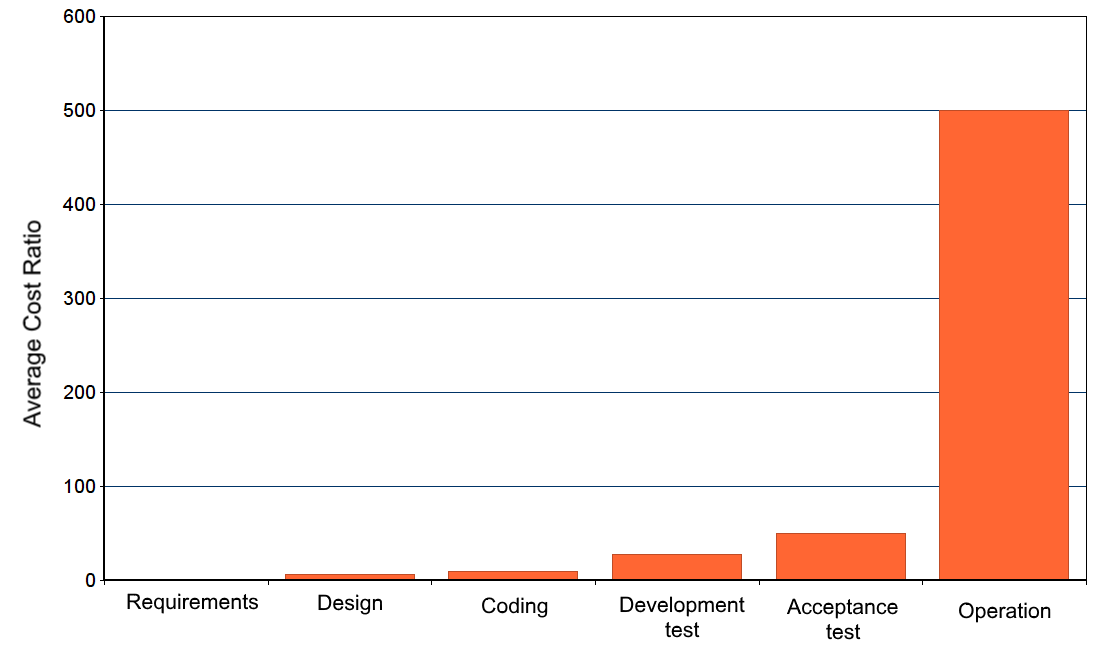
\includegraphics[,width=4in]{b81.png}
 \end{center}
 \caption{A widely-recreated chart of the DIE effect. Adapted from Boehm'81~\cite{Boehm81}. }\label{fig:b81}
 \end{figure}

Like any good theory, DIE includes a rationale for why the expected results would be seen. McConnell mentions it as a ``common observation'' in the field and  summarizes the intuitive argument for why it should be so: 
\begin{quote}
''A small mistake in upstream work can affect large amounts of downstream work. A change to a single sentence in a requirements specification can imply changes in hundreds of lines of code spread across numerous classes or modules, dozens of test cases, and numerous pages of end-user documentation''~\cite{mcconnell01}. 
\end{quote}
Glass also endorses this rationale, asserting that ``requirements errors are the most expensive to fix when found during production but the cheapest to fix early in development'' is ``really just common sense''~\cite{glass02}.  Other researchers
are just as adamant in asserting that that the delayed issue effect is a generally useful law of software engineering.
For example, what we call the delayed issued effect was listed at \#1 by Boehm and Basili in their ``Top 10 list'' of ``objective and quantitative data, relationships,
and predictive models that help
software developers avoid predictable pitfalls
and improve their ability to predict
and control efficient software projects''~\cite{boehm01}.
  
In analyzing data from a contemporary set of software development projects, however, we did not find results to corroborate these claims. While the delayed issue effect might have been a dominant
effect decades ago, this does not mean that it is necessarily so for $21^{\mathit{st}}$ century
software development. 
 The delayed issue effect was first reported in 1976 in a era of punch card programming
and non-interactive environments~\cite{Boehm76}. In the 21$^\mathit{st}$ century, we  program in 
interactive environments with higher-level languages and better source code control
tools. Such tools allow for the faster refactoring of existing
code-- in which case, 
managing the changes required to fix (say) an incorrect requirements assumption
is far less    onerous    than before. Further, software engineering theory and practice has evolved into new paradigms focused on rapid feedback and delivery, enabled by significant technological advances in the past 40 years. There is little empirical evidence for the delayed issue effect since its initial observation, no doubt due in part to DIE being ``just common sense'' as Glass states~\cite{glass02}. 

This article explores the currency of the delayed issue effect.
% Given all of the changes to development practice in the time since the effect was first observed, finding no softening of the DIE might be taken as more surprising than our current results. These changes in software development practice are discussed later in this paper.
% The above argument is an anecdotal evidence that  the delayed issue effect might no longer exist. But anecdotes are not rigorous
% evidence. Accordingly,  this article explores the currency of the delayed issue effect.
After some initial definitions, we discuss the
value of checking old ideas. Next, we present a survey of industrial practitioners and researchers that documents the widespread belief that delayed issues have a negative impact on projects.  After that, we  analyze 171 software  projects developed in the period 2006--2014 and find  {\em no evidence} of the delayed issue effect. Finally, we discuss the validity and implications of our results, as well as possible reasons for the lack of observed effect given the state of the practice - reasons which, when subjected to further testing, may prove useful for refining the theory. To ensure reproducibility,
all the data  used in this study is available in the PROMISE
repository at openscience.us/repo. 
To the best of our knowledge,
this the largest study devoted the delayed issue effect yet conducted.




\subsection{Preliminaries}\label{sect:nontsp}
Before beginning, it is appropriate to make the following full disclosure statement. 
All 171 software projects
studied here were developed using the Team Software Process (TSP$\textsuperscript{SM}$), which is a software development methodology
developed and promulgated by the employer of the second and third author of this paper (for more details on TSP,
 see \tion{tsp}).

We argue that TSP is not such a radical change to software development that it can
stamp out a supposedly rampant problem like the delayed issue effect. We view TSP as a better way to
 {\em monitor} the activities   of  existing projects.  TSP
 does not significantly change a project-- it just offers a better way to log the activity within
 that project. The limitations of our sample drawing from TSP projects are discussed more thoroughly in the Threats to Validity section. 
 
% Hence, given our data, the conclusion of this paper is {\em  either} the delayed issue effect can be  removed via:
% simple changes to a project (like TSP) {\em or} that the DIE problem does not exist in the first place, on at least some class of projects.
% Either way, our  general point is the same: the delayed issue effect is not useful as a general law of what can be expected from software development practice. 

 





 
\section{Definitions \& Claims}
\label{sect:claims}

This paper uses the following definitions:
\bi
\item
The {\em delayed issue effect}:   it is {\em very much}  more {\em difficult} to resolve  issues in a software project, the {\em longer} they remain.
\item
 {\em Longer} time is defined as per  Boehm'81~\cite{Boehm81}; i.e. the gap between the   phases where   issues are introduced and resolved.
\item
We say that a measure $m$ collected in phase ${1,.,i,..j}$ is 
{\em very much} more when  that
   measure at phase $j$   
   is larger than the sum of those measures in the earlier phases;
   i.e. $\sum_{i=1}^{j-1} m_i $. 
\item
Issues are more {\em difficult}  
when their resolution takes more time or costs more  (e.g. needs expensive
debugging tools or the skills of expensive developers).
\ei
% Note that we use  the  term ``delayed issue effect'' as generalization of the
% more specific rule  ``requirements errors are hardest to fix''.
% This generalization is valid since the rationale for the rule about requirements
% is usually done as per McConnell~\cite{mcconnell01}; i.e. small upstream mistakes very
% early in the system can cascade into huge problems later in the lifecycle.
% That said, we prefer our more general term ``delayed issue effect'' since not
% only might requirements errors cascade, so too might analysis errors, design errors, etc.


Note that this  definition of ``difficult to resolve''  combines two concepts: time to change and cost to change.  Is it valid to assume the equivalence of time and cost?
Certainly, there are cases where time is not the same as cost. Consider, for example, if debugging required some very expensive tool or the services or a very senior (and hence, very expensive) developer. Under those circumstances, time does not equate to cost.
Having documented the above issues, we assert that they are unlikely to be major issues in the study. One of us (Nichols) was closely associated with many of the projects in our sample. He is unaware of any frequent use of exorbitantly expensive tools or people on these projects. For more on the validity of this definition
of ``difficult to resolve'' see \tion{construct}.



This paper defends the following claim and hypothesis. The hypothesis is defended
using some statistical
significance tests while the claim is supported via a variety
of arguments.

{\bf  Claim: ``DIE'' is a  commonly held, yet poorly documented belief.}
We examine the literature promoting the DIE and find that most reference a few primary sources. Many of the papers reporting the DIE
 either (1)~are quite old (papers dating from last century);
(2)~quote prior papers without presenting   new data; 
(3)~or cite data sources that can no longer be
confirmed. We follow-up with a short survey that finds that DIE appears as the most strongly-held belief among software engineers in our sample. 


{\bf Hypothesis: Delayed issues are not harder to resolve.}
 In our sample of 
 171 commercial software  projects, we offer  a statistical analysis showing that, in overwhelming majority
 of our results, there is no   
 significant increase in the time to resolve issues  as they are delayed across multiple phases.
 


 
 


\section{ Reassessing Old Truisms}
General
theories of software
engineering principles are common to both research and practice, although not always explicitly stated. Such theories underlie  lists of proposed general ``best practices'' for effective software development, such as
the IEEE 1012 standard for software verification~\cite{1012}. 
 Endres \& Rombach offer empirical observations, theories, and laws\footnote{Endres \& Rombach note that these are not laws of nature in the scientific sense, but theories with repeated empirical evidence.}~\cite{endres03}.
 Many other 
commonly cited researchers  do the same, e.g.,
Glass~\cite{glass02}, Jones \cite{jones07}, and Boehm~\cite{boehm00b}.
Budgen \& Kitchenham seek to reorganize SE research using
general
conclusions drawn from a larger number of studies~\cite{kitch04,budgen09}.

In contrast, there are many empirical  findings 
that demonstrate the difficulty in finding general truisms in software engineering, even for claims that seem intuitive:

\be
\item
Turhan~\cite{me12d} lists 28 studies with contradictory conclusions
on the relation of object-oriented (OO) measures to defects.  Those results
 directly  contradict some of the laws listed by 
Endres \& Rombach~\cite{endres03}.
\item
Ray et al.~\cite{ray2014lang} tested if   strongly typed languages
predict for better code quality. In  728 projects,
they found  only a modest benefit in strong typing and warn that the effect may be due to other conflating factors.
\item
Fenton \& Neil~\cite{fenton00,fenton00b}   critique the truism that
``pre-release fault rates for software
are a predictor for post-release failures'' (as claimed in~\cite{dunsmore88},
amongst others). For the systems described in~\cite{fenton97}, they
show that software modules that were highly fault-prone
prior to release revealed very few faults after release.
% \item
% Meyer claims that OO encapsulation will
% reduce error rates in software~\cite{Meyer1988}.  Yet empirical results suggest
% that debugging an OO program is many times harder and
% longer than debugging a standard procedural program~\cite{hatton98}.
% \item
% A truism of visual programming is that ``visual
% representations are inherently superior to mere textual representations''. A review by Menzies suggests that the available
% evidence for this claim is hardly conclusive~\cite{me00v}. 
\item
Numerous recent {\em local learning} results compare single models
learned from all available data to multiple models learned from clusters within the data~\cite{betten14,yang11,yang13,minku13,me12d,me11m,betta12,posnett11}.
A repeated result in those studies is that the local models generated the better effort
and defect predictions (better median results,
lower variance in the predictions).
\ee
 
The dilemma of failing truths in the face of new evidence is not particular to software engineering. 
% To be fair, 
% SE is  not the only
% field where practitioners hang on to persistent beliefs, even if the evidence
% for those beliefs is not strong.
The medical profession applies  many practices based on studies
that have been disproved. For example,
a  recent article
in the Mayo Clinic Proceedings~\cite{prasad13} found  
146 medical practices based on studies 
in year $i$, but which were  reversed by subsequent trials within years $i+10$.
Even when the evidence for or against a treatment or intervention is clear, medical providers and patients may not accept it~\cite{aschwanden10}.
Aschwanden warns that ``cognitive biases''  such as  confirmation bias (the tendency to look for evidence that supports what you already know and to ignore the rest)  influence how we process information~\cite{aschwanden15}.

The cognitive issues that complicate medicine are also found in software engineering.
Passos et al.~\cite{passos11} warn that developers
usually develop their own theories of what works and what doesn't work in creating software, based on experiences from a few past
projects. Too often, these theories are assumed to be general truisms with widespread applicability to future projects. They comment ``past experiences were taken into account without 
much consideration for their context''~\cite{passos11}.
The results of J{\o}rgensen \& Gruschke~\cite{jorgensen09} support Passos et al. In an empirical study of expert effort estimation, they report that the experts rarely use lessons
  from past projects to improve their future reasoning in effort estimation~\cite{jorgensen09}. 
 They note that,
when the experts
  fail to revise their beliefs, this leads to poor
 conclusions and software projects  (see examples in~\cite{jorgensen09}).
 A similar effect is reported by
Devanbu et al.~\cite{prem16}  who examined responses from 564 Microsoft software developers from around
the world, they found that  ``(a)~programmers do indeed have very
strong beliefs on certain topics; (b)~their beliefs are primarily formed
based on personal experience, rather than on findings in empirical
research; (c)~beliefs can vary with each project, but do not necessarily
correspond with actual evidence in that project''.
Devanbu et al. further  comment that ``programmers give personal experience
as the strongest influence in forming their opinions''. This is a troubling
result, especially given the above comments from Passos and  J{\o}rgensen et al.~\cite{passos11,jorgensen09} about how quickly practitioners form, freeze, and rarely revisit those opinions.

 
 
From all we above we conclude that, just as in medicine, 
%our field suffers when
 %software engineers do  not revise old beliefs.  Therefore, 
 it is important for our field
 to regularly  reassess old truisms  like the  delayed issue effect.
  
 
 
\section{Motivation: ``DIE'' is commonly held, yet poorly documented}
\label{sect:belief}
% To assess the prevalence of DIE,   we conducted a survey of software engineers. If our surveyed practitioners make management decisions based on their
% understanding of SE theory, then the DIE  may well influence their decisions.
One reason that industrial practitioners and academics believe so strongly in the delayed issue effect is that it is often referenced
in the SE literature. 
%For example,
%we know that \fig{b81} has been presented to the graduate SE class at North Carolina State University, without quarrel or %critical comment, every year for the last decade.
Yet when we look at the literature, the evidence for
delayed issue effect is both very sparse and very old.

We examined the literature on the delayed issue effect through a combination of snowball sampling~\cite{wohlin2014guidelines} and database search. We searched Google Scholar for terms such as ``cost to fix'' and ``defect cost'' and ``software quality cost''. The majority of the search results discuss quality measurements, quality improvement, or the cost savings of phase-specific quality improvement efforts (e.g., heuristic test case selection vs. smoke testing). A systematic literature review of software quality cost research can be found in \cite{karg2011systematic}. Relatively few articles discuss cost-to-fix as a function of when the defect was injected or found. We also conducted a general Google search for the above terms. We found a number of website articles and blog postings on this topic, e.g., \cite{IfSQ2013,Soni2016,Parker2013,Gordon2016}. From these, we gathered additional citations for the delayed issue effect, the vast majority of which were secondary sources, e.g.,~\cite{Leffingwell96,mead2004software,mcconnell1996software,mcconnell01,Tassey2002,boehm2012}. Our literature search is not exhaustive, but our results yielded an obvious trend: nearly every citation to the delayed issue effect could be traced to the seminal \textit{Software Engineering Economics}~\cite{Boehm81} or its related works~\cite{boehm88,boehm01}.\footnote{For example, popular sources such as~\cite{pressman2005software, boehm01,glass02,endres03} have a combined citation count of over 14,500 on Google Scholar can all trace their evidence to \textit{Software Engineering Economics}~\cite{Boehm81}.}


Ultimately, we identified nine sources of evidence for the delayed issue effect based on real project data: the original four \cite{Fagan76,Boehm76,Daly77,Stephenson76} reported in \textit{Software Engineering Economics}\cite{Boehm81}, a 1995 report by Baziuk~\cite{baziuk1995bnr} on repair costs at Nortel, a 1998 report by Willis et al.~\cite{willis1998hughes} on software projects at Hughes Aircraft, a 2002 experiment by Westland~\cite{westland2002cost} to fit regression lines to cost-to-fix of localization errors, a 2004 report by Stecklein et al.~\cite{steck04} on cost-to-fix in five NASA projects, and a 2007 survey by Reifer on CMMI Level 5 organization\cite{reifer2007profiles}.







\begin{figure}[!t]
% \begin{center}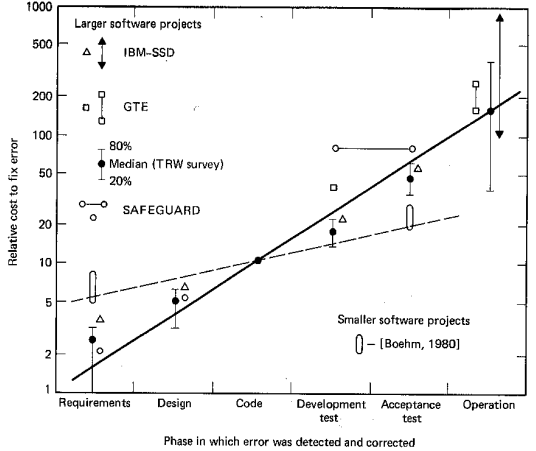
\includegraphics[width=4in]{boehm_cost-to-fix.png}\end{center}
\begin{center}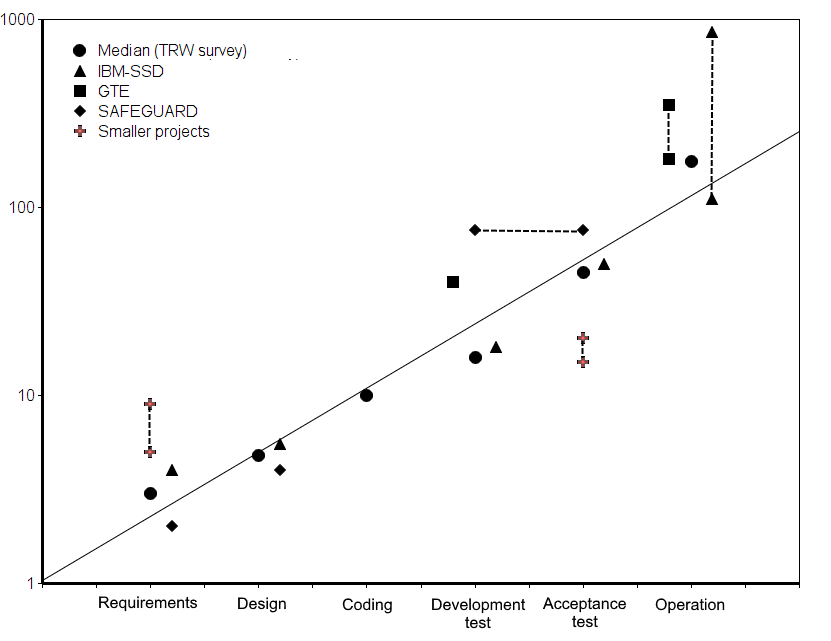
\includegraphics[width=4.5in]{boehm81.png}\end{center}
 \caption{Historical cost-to-fix curve. Adapted from~\cite{Boehm81}, p. 40.}\label{fig:cost-to-fix}
 \end{figure}

Figure~\ref{fig:cost-to-fix} shows the DIE as reported in \textit{Software Engineering Economics}~\cite{Boehm81} based on data from large systems in the late 70s from IBM~\cite{Fagan76}, TRW~\cite{Boehm76}, GTE~\cite{Daly77}, and Bell Labs~\cite{Stephenson76}. 
%These studies are most often cited by secondary sources on the delayed issue effect (e.g., \cite{boehm01, mcconnell01,glass02}. 
We note that it is unclear from the text in~\cite{Daly77} and \cite{Boehm76} if cost is defined in terms of effort, or in actual cost (i.e., labor, materiel, travel, etc). The data points from these studies are not published for analysis.
Baziuk~\cite{baziuk1995bnr} reports an exponential increase in the cost to patch software in the field versus system test, and Stecklein et al.~\cite{steck04} produce a cost-to-fix curve (as price) that fits precisely with \fig{cost-to-fix}. Westland~\cite{westland2002cost} finds that the cost to fix engineering errors is exponentially related to the cost of the overall cost of a case study project. Reifer~\cite{reifer2007profiles} confirms the exponential increase in the DIE in 19 CMMI Level 5 organizations though this appears to be based on survey rather than empirical data. 

% \begin{figure}[!ht]
% \centering
% \begin{tabular}{lllll}
%                 &   Inception   &   Elaboration &   Construction    &   Transition  \\\hline
% Inception       &   25-100      &               &                   &               \\
% Elaboration     &   100-500     &   50-250      &                   &               \\
% Construction    &   500-1,000   &   250-1,500   &   75-500          &               \\
% Transition      &   8,000-10,000  &  1,500-5,000   &   500-3,000        &   Not enough data\\
% \end{tabular}
% \caption{Range of cost to find and fix defects (\$US per defect) from~\cite{reifer2007profiles}.}
% \label{fig:reifer}
% \end{figure}





 

Shull et al.~\cite{Shull02} conducted a literature survey and held a series of e-workshops with industry experts on fighting defects. Workshop participants from Toshiba and IBM reported cost-to-fix ratios between early lifecycle and post-delivery defects of 1:137 and 1:117 for large projects respectively~\cite{Shull02} -- but the raw data points were not provided and thus cannot be confirmed. A goal of agile methods 
is to reduce the difficulty associated with making changes later in the lifecycle~\cite{beck00}. Relatively little empirical data exists on this point.
Elssamadisy and Schalliol~\cite{Elssamadisy02} offer an anecdotal report on the growing, high cost of rework in a 50 person, three-year, 500KLOC Extreme Programming project as the project grew in size and complexity-- but again we cannot access their 
exact figures. This was a common theme in the literature reviewed for this paper-- i.e.  that  it was no longer possible to access the data used to make prior conclusions. 





 
% We note that previous work focuses on cost-to-fix as a function of lifecycle phase irrespective of when the defect was injected, that is, previous work analyzes the cost to fix a defect found in test regardless of whether that defect was a requirements error or a coding mistake. To our knowledge, our research represents the first large-scale study of phase delay.





% \begin{figure}[!t]
% \begin{center}
%  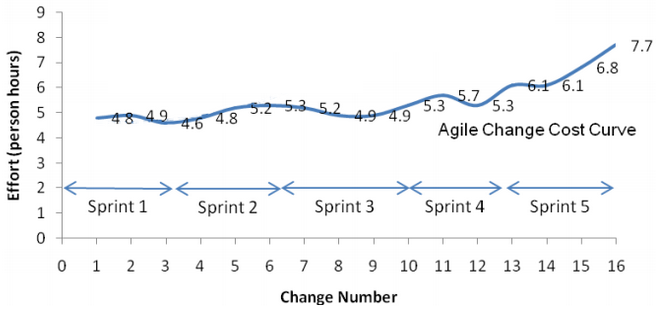
\includegraphics[width=4in]{img/clutterbuck.png} 
%  \end{center}
%  \caption{Cost of change from an agile case study. From~\cite{Clutterbuck09}.}\label{fig:clutterbuck}
%  \end{figure}

 
 
 %  All in all, the literature reviewed in this section
% does not inspire confidence in a DIE effect due
% to a lack of applicability and lack of replication.
%  Adding to our doubts are  
 
% Clutterbuck et al.~\cite{Clutterbuck09} studied a 5-month effort by a small-to-medium enterprise team developing a 71KLOEC web interface to a database application to implement 18 change requests-- see Figure~\ref{fig:clutterbuck} (note that these were for new and changed user requirements, not defects). Clutterbuck et al. found the cost of change to be relatively flat until the later phases, with much of the effort spent in analysis of the change requests~\cite{Clutterbuck09}. Note that in this study, the effort increased by only 60\% (see the start and end of the curve in Figure~\ref{fig:clutterbuck}).




 
Some studies that report less-than large
 increase in the effort required to fix delayed issues.  Boehm~\cite{Boehm80} provides data suggesting that the cost-to-fix curve for small projects
 %, two student projects of 2000 deliverable source instructions, 
 is flatter than for large projects (the dashed line of Figure~\ref{fig:cost-to-fix}). Data from NASA's Johnson Space Flight Center, reported by Shull~\cite{Shull02}, found that the cost to fix certain non-critical classes of defects was fairly constant across lifecycle phases (1.2 hours on average early in the project, versus 1.5 hours late in the project). Royce~\cite{Royce98} studied  a million-line, safety-critical missile defense system. Design changes (including architecture changes) required approximately twice the effort of implementation and test changes, and the cost-to-fix in implementation and test phases increased slowly. Boehm~\cite{Boehm10} attributes this success to a development process focused on removing architecture risk early in the lifecycle. Willis et al. (\cite{willis1998hughes}, page 54) provide tables summarizing the effort to fix over 66,000 defects as a function of lifecycle phase injected and removed from multiple projects. The tables are partly obscured, but seem to provide the first large scale evidence that a)~DIE need not be exponential and b)~DIE need not be monotonically increasing.  Again, the data points from these studies are not available, and thus newer evidence both in favor of and contrary to the DIE cannot be evaluated.




To gain a sense of how current the perception of the DIE is, 
we conducted two surveys of software engineers. 
The surveys collected data on software engineers' views of the DIE and other commonly held software engineering ``laws''. The surveys were conducted using Amazon's Mechanical Turk. The first survey was conducted only with professional software engineers. Participants were required to complete a pretest to verify their status as a professional or open source software developer and to confirm their knowledge of basic software engineering terminology and technology. The  second survey was conducted with Program Committee members of the ESEC/FSE 2015 and ICSE 2014 conferences solicited via email.

The practitioner survey presented the following law: ``requirements errors are the most expensive to fix when found during production but the cheapest to fix early in development'' (from Glass~\cite{glass02} p.71 who references Boehm \& Basili~\cite{boehm01}). We abbreviate this law as RqtsErr.\footnote{We use the RqtsErr formulation since this issue typically needs no supportive explanatory
text. If we had asked respondents about our more general term ``delayed issue
effect'', we would have had to burden our respondents with extra explanations.}
The PC member survey presented the RqtsErr law and an additional law on the DelayedIssueEffect: ``In general, the longer errors are in the system (requirements errors, design errors, coding errors, etc.), the more expensive they are to fix''.  The respondents answered two questions in response to each law:
\bi
\item \textbf{Agreement:} ``Based on your experience, do you agree that the statement above is correct?'' A Likert scale captured the agreement score from Strongly Disagree to Strongly Agree. A text box was provided to explain the answer. 
\item \textbf{Applicability:} ``To the extent that you believe it, how widely do you think it applies among software development contexts?'' The possible answers were: -1: I don't know, 0: this law does not apply at all, ..., 5: always applies. Respondents were required to explain the applicability score in a text box.
\ei

\begin{figure}[ht] 
\scriptsize 
 \begin{center}
\begin{tabular}{l|c|c|c|c|c}
 &  & \multicolumn{2}{c|}{agreement} & \multicolumn{2}{c}{applicability} \\
Practitioner survey  & N & med & mode & med & mode \\
\hline 
\textbf{Rqts errors are most expensive...} & 16 & 5 & 5 & 4 & 5 \\ 
Inspections can remove 90\% of defects & 18 & 4 & 5 & 4 & 5 \\
80-20 rule (defects to modules) & 12 & 4 & 5 & 4 & 5 \\
Most time is spent removing errors & 16 & 4 & 4 & 4 & 5 \\ 
Process maturity improves output & 17 & 4 & 4 & 4 & 4 \\ 
Missing reqts are hardest to fix & 17 & 4 & 4 & 4 & 4 \\
Reuse increases prod. and qual. & 16 & 4 & 4 & 4 & 4 \\
OO-programming reduces errors & 13 & 4 & 4 & 4 & 3 \\
Adding manpower to a late project & 15 & 4 & 4 & 4 & 4 \\
Smaller changes have higher error density & 14 & 3 & 3 & 3.5 & 5 \\
A developer is unsuited to test own code & 17 & 3 & 1 & 4 & 5\\
 \multicolumn{6}{l}{}\\
\multicolumn{6}{l}{Researcher survey} \\\hline 
Process maturity improves output & 4 & 4 & 4 & 4 & 5 \\
\textbf{Rqts errors are most expensive...} & 30 & 4 & 4 & 4 & 4   \\ 
\textbf{DelayedIssueEffect} & 30 & 4 & 4 & -- & --  \\
Reuse increases prod. and qual. & 6 & 4 & 4 & 4 & 4 \\
80-20 rule (defects to modules) & 6 & 4 & 4 & 4 & 3 \\
Missing reqts are hardest to fix & 7 & 4 & 4 & 4 & 3 \\
OO-programming reduces errors & 6 & 4 & 4 & 3 & 4 \\
Inspections can remove 90\% of defects & 7 & 4 & 4 & 3 & 3 \\
Adding manpower to a late project & 4 & 3 & 4 & 4 & 3 \\
Most time is spent removing errors & 6 & 3 & 3 & 4 & 4 \\ 
Smaller changes have higher error density & 4 & 3 & -- & 4 & 4 \\
A developer is unsuited to test own code & 7 & 2 & 1 & 3 & 3
\end{tabular} 
 \end{center}
\caption{Agreement and applicability of SE axioms.}
\label{fig:survey_results}
\end{figure}

Summary statistics for the agreement and applicability scores for the RqtsErr and DelayedIssueEffect laws are presented in Figure~\ref{fig:survey_results}. Responses whose Applicability response was ''I don't know'' are omitted from analysis. Laws other than RqtsErr and DIE are not relevant to this paper, but are shown for comparison.  


Both  practitioners and researchers strongly believed in RqtsErr. In both sets of responses, RqtsErr received  scores higher than most
other laws. Overall, the RqtsErr law was the most agreed upon and most applicable law of 11 surveyed amongst practitioners, and the second most agreed upon law amongst researchers. From the free response texts, we note that the researchers who disagreed with RqtsErr generally asserted that requirements change can be expensive, but that the effect depends on the process used (e.g., agile vs. waterfall) and the adaptability of the system architecture.

The above arguments provide evidence to the claim that the DIE is both poorly documented yet (still) widely believed. The comments of Glass~\cite{glass02}, that the DIE is ``just common sense'', suggest that DIE may be the target of confirmation bias. An example of this is \fig{steck} from~\cite{steck04}, which purports to show nine references to ``studies [that] have been performed to determine the software error cost factors''. Only one of these sources, \textit{Software Engineering Economics}~\cite{Boehm81}, is based on real project data.  Despite a lack of recent evidence, the perception of the DIE persists today among both the software engineers sampled in our survey and in popular literature. In the intervening years, many advances in software technology and processes have been made precisely to deal with risks such as the DIE. Thus, it is appropriate to ask the question, does the DIE still exist?

 \begin{figure}[!ht] 
{\small
\begin{center}
\begin{tabular}{r|rrrr|l}
                        & \multicolumn{4}{c}{Phase Requirements Issue Found }   &     \\
 Cited source           & Requirements  &   Design  &   Code    &  Test         & Data sources used to determine DIE          \\\hline
\cite{Boehm81}          &   1           &   5       &   10      &   50          & Multiple projects     \\  
Hoffman, 2001           &   1           &   3       &   5       &   37          & Unknown - no bibliography entry \\ 
\cite{Cigital2003}      &   1           &   3       &   7       &   51          & Extrapolated from defect counts for a one project \\
\cite{Rothman2000}      &               &   5       &   33      &   75          & Fictitious example \\
\cite{Rothman2000} Case B   &               &           &   10      &   40      & Fictitious example \\
\cite{Rothman2000} Case C   &               &           &   10      &   40      & Fictitious example \\
\cite{Rothman2002}      &   1           &   20      &   45      &   250         & Fictitious example \\
\cite{Pavlina2000}      &   1           &   10      &   100     &   1000        & None provided \\
\cite{McGibbon2007}     &               &   5       &           &   50          & Pen \& paper exercise - no real data \\
\end{tabular}
\end{center}}
\caption{Confirmation bias -- sources for DIE cited in Table 1 of~\cite{steck04}. Note that \textit{all} of these are cited as ``studies [that] have been performed to determine the software error cost factors'', but only one, \cite{Boehm81}, is backed by actual data.}\label{fig:steck}
\end{figure}




% \begin{figure}
% \begin{center}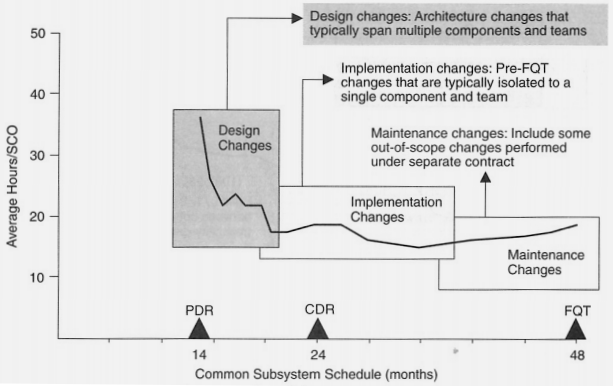
\includegraphics[width=4in]{img/Royce98.png}\end{center}
%  \caption{Exception to the rule - The Royce study: cost-to-fix curve. From~\cite{Royce98}.}\label{fig:royce}
%  \end{figure}

\subsection{Early Onset of the DIE Effect}\label{sect:earlyonset}

One feature of the the DIE literature is important to our subsequent discussion:   
the onset of  DIE  {\em prior} to delivery.
\bi
\item  
\fig{b81} reports a 40-fold increase in effort requirements to acceptance testing
\item
 \fig{cost-to-fix} reports a 100-fold increase
(for the larger projects) before the code is delivered 
\ei
Any manager noticing this  early onset of DIE (prior to delivery, during the initial development)
would be well-justified
in believing that  the difficulty in resolving issues  will get much worse. Such managers
would therefore expect DIE to have a marked effect post-deployment.
We make this point since,  in the new project data presented below, we focus on DIE pre-delivery.
%there is no early onset of DIE. 
% That is:
% \bi
% \item There is no evidence of a growing problem prior to delivery that delayed issues are becoming harder to manage
% \item  Hence, there is less evidence that DIE is a trend that will significantly and negatively effect the product,
% post-delivery.
% \ei


 

\section{Delayed Issues are not  Harder  to Resolve}
\label{sect:analysis}
The above analysis motivates a more detailed look at the delayed issued effect.  
Accordingly, we examined 171 software projects conducted between 2006 and 2014. 

These projects took place at organizations in many countries and were conducted using  the Team Software Process (TSP$\textsuperscript{SM}$). Since 2000, the SEI has been teaching and coaching TSP teams. One of the authors (Nichols) has mentored software development teams and coaches around the world as they deploy TSP within their organizations since 2006.  The  most recent completions were in 2014.

The projects were mostly small to medium, with a median duration of 46 days and a maximum duration of 90 days in major increments. 
Several projects extended for multiple incremental development cycles. 
Median team size was 7 people, with a maximum of 40. See \fig{dist} for the total
effort seen in those projects. Many of the projects were e-commerce web portals or banking systems in the US, South Africa, and Mexico. 
There were  some  medical device projects in  the US, France, Japan, and Germany as well  as a commercial computer-aided design systems, and embedded systems. A more thorough characterization of the projects providing data is provided in \S\tion{data_character}.

An anonymized version of that data is available in the PROMISE repository at openscience.us/repo.
For confidentiality restrictions, we cannot offer 
further details on these projects.

\subsection{About TSP$\textsuperscript{SM}$}\label{sect:tsp}

TSP is a software project management approach developed at the Software Engineering Institute (SEI) at Carnegie Mellon University~\cite{tsp00}. TSP is an extension of the Personal Software Process (PSP$\textsuperscript{SM}$) developed at the SEI by Watts Humphrey~\cite{tsp00}.  
 

%TSP helps developers via a set of measures that can be applied to managing tasks, quality, and schedule. Planning begins by quantifying goals, defining work practices, and estimating size and effort. Developers then use this information to make a detailed short term plan. As the developers perform project work, they use a tool such as the Process Dashboard to collect their time, effort, size, and schedule data. Every week, the team reviews their data to evaluate status, identify actual rates, determine if project goals for schedule, cost, and quality are being met. The team then uses this information to make necessary plan corrections. At the end of the project the coach and team perform a quantitative project post mortem.

Common features of TSP projects include {\em planning}, {\em personal reviews}, {\em peer inspections}, and {\em coaching}.
A TSP {\em coach} helps the team to plan and analyze performance. The coach is the only role authorized to submit project data to the SEI.
Before reviewing data with the teams, therefore before submission, these coaches check the data for obvious errors.

During {\em Planning}, developers estimate the size of work products and convert this to a total effort using historical rates. Time in specific tasks come from the  process phases and historical percent time in phase distributions. Defects are estimated using historical phase injection rates and phase removal yields. Coaches help the developers to compare estimates against actual results. In this way, developers acquire a more realistic understanding of their work behavior, performance, and schedule status.

{\em Personal review} is a technique taken from the PSP and its use in TSP is unique.  Developers follow a systematic process to remove defects by  examining their own work products using a checklist built from their personal defect profile. This personal review occurs after some product or part of a product is considered to be constructed and before peer reviews or test. 

%PSPSM teaches developers howto continually make and review their personnel estimates
%about their day-to-day tasks, then compare those estimates against the actual development effort.
%In this way, developers can acquire a more realistic understanding of their work behaviour.
  
 
 
\begin{figure}
\begin{center} 
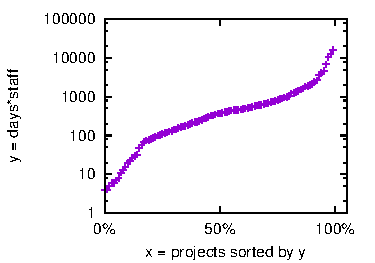
\includegraphics[width=2.5in]{dom.pdf}
\end{center} 
\caption{Distribution of 
{\em effort} (which is
{\em team size} times
{\em days of work}). For example, if 10 programmers work for 10 days,
then the effort is 100 days. The median value in this plot
 271 days.}\label{fig:dist}
\end{figure}

{\em Peer inspection} is a  technique in
traditional software engineering and is often called peer review.
 Basili and Boehm   commented in 2001~\cite{boehm01} 
that peer reviews can catch over half the defects introduced into a system.
Peer inspection can be conducted on any artifact generated anywhere in the software
lifecycle and can quickly be adapted to new kinds of artifacts. TSP peer reviews follow the Fagan style in which the reviewer uses a checklist composed of common team defects prior to a review team meeting. 
 
Overall, the   effort associated with adding TSP to a project is not onerous. McHale reports~\cite{mchale02}:
\bi
\item
 The time spent  tracking time, defects, and tasks requires less than 3\% of a developer's time. Weekly team meetings  require at most an hour, which is
only 2.5\% of a 40 hour work week. 
\item
Team launches and replans average about 1 day per month or 5\% planning overhead.
\ei
It is true that one staff member is needed as a ``coach'' to mentor the teams
and certify and monitor that data collection. However, one of us (Nichols) has worked with dozens of TSP teams. He reports that one  trained coach can support 4 or 6 teams (depending upon team experience).
 




\subsection{Data Collection and Definitions}
\label{sect:data-collection}

Organizations using TSP agree to provide their project data to the SEI for use in research. In return the SEI agrees that  data must not be traceable to its source. The data is collected at major project events: launch, interim checkpoints, and at project completion. The data from these TSP projects were collected and stored in the Software Engineering Measured Process Repository (SEMPR) at the SEI. 

As of November 2014, the SEI TSP database contained data from 212
TSP projects. The projects completed between July 2006 and
November 2014; they included 47 organizations and 843 people. 
The database fact tables
contain 268,726 time logs, 
154,238 task logs,
 47,376 defect logs, 
and 26,534 size logs. 
In this paper, we exclude 41 of the 212 that had too few defects (less than 30), leaving 171 projects included in the analysis.

% Data includes project and site  characteristic summaries, surveys of team members, launch presentations, launch outbriefs, and baseline plans, final data from the project, and the project post mortem report.  In practice, this data requirement has only been enforced for the purposes of certifying and reauthorizing TSP coaches who must submit data to maintain their authorization. Coaches are certified by demonstrating competent use of the TSP process with the artifacts and data not by the actual project results.  Of the data submitted, only the data recorded using the Process Dashboard tool has been collected and aggregated for this research. 
 %The key views include a project results summary, effort logs, task logs, and defect logs. The data has not yet undergone additional screening. A summary of the data quality issues was reported in a previous work ~\cite{shirai14} (that summary is discussed further in our {\em Validity} section, below).
 
% Our units of analysis are: \textit{time}, \textit{defects}, \textit{time per defect}, and \textit{phase of development}.

% \bi
%     \item \emph{defects} - individual defects are recorded as line items in the defect logs uploaded to the SEMPR at the SEI. One or more defects are reported against a single \emph{plan item} in the time tracking logs, e.g., a review session, an inspection meeting, a test execution.
%     \item \emph{time} - Time is tracked per person per plan item in the time-tracking logs, e.g. a 30 minute design review session involving 3 people will have three time log entries summing to 90 minutes. Time includes the time to analyze, repair, and validate a defect fix.
%     \item \emph{time per defect} - The total \# of defects found in a plan item during a removal phase divided by the total time spent on that plan item in that phase.
% \ei

\subsubsection{Definition: time for plan item}

Using a tool supporting the SEI data specification, developers keep detailed time-tracking logs. The time-tracking logs record  work start time, work end time,  delta
work time, and interruption time. Software engineers are often
interrupted by meetings, requests for technical help, reporting, and
so forth. These events are recorded, in minutes, as interruption
time. In TSP, time logs are recorded against \textit{plan items}. A planned item is a specific task assigned to a specific developer, such as resolving a defect, coding a feature, performing an inspection or writing a test. Each  work session includes a start time, an end time, and interruption time. The active time, or actual time for the plan item is calculated by summing the active time durations for all work sessions on that task.
\[
\text{\emph{actual time for plan item}} := \text{SUM(}\text{end time} - \text{start time} - \text{interruption time}) 
\]
Time is tracked per person per plan item in the time-tracking logs, e.g. a 30 minute design review session involving 3 people will have three time log entries summing to 90 minutes. Time includes the time to analyze, repair, and validate a defect fix.

% In this paper, when we report ``time to resolve an
% issue,'' we show the difference between the start and end times
% of a work session, with any interruption time subtracted (the
% difference in times, minus the interruptions). 


\subsubsection{Definition: defects and time-to-fix}\label{sect:defin}
In the TSP, a  \emph{defect} is any change to a product, after its construction, that is necessary to make the product correct.  A typographical error found in review is a defect. If that same defect is discovered while writing the code but before review, it is not considered to be a defect. 
SEI TSP defect types are:
\bi
\item Environment: design, compile, test,  other support  problems
\item Interface: procedure calls and reference, I/O, user format
\item Data: structure, content
\item Documentation: comments, messages
\item Syntax: spelling, punctuation typos, instruction formats
\item Function: logic, pointers, loops, recursion, computation  
\item Checking: error messages, inadequate checks
\item Build: change management, library, version control
\item Assignment: package
declaration, duplicate names, scope
\item System: configuration, timing, memory
\ei

\begin{figure}[t]
\begin{center}
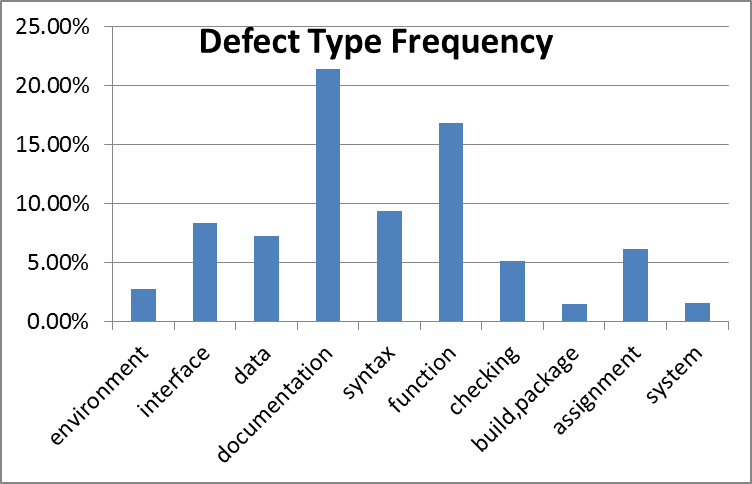
\includegraphics[width=2.5in]{defect_type_frequency.png}
\end{center}
\caption{Relative frequencies of these defect types seen in our TSP data.}\label{fig:dtypes}.
\end{figure}
In our TSP data,  the relative frequencies of these defect types are shown in \fig{dtypes}. Around a quarter of the fixes were simple documentation changes.
That said, 75\% of the changes are quote  elaborate;   e.g. fixes to function necessitates a careful reflection of the purpose of the code.

Individual defects are recorded as line items in the defect logs uploaded to the SEMPR at the SEI. The defect entry includes the time and date a defect was discovered, the phase in which that defect was injected, the development phase in which it was removed, the time (in minutes) required to find and fix the defect, and the categorical type. 

One or more defects are reported against a single plan item in the time tracking logs, e.g., a review session, an inspection meeting, a test execution. The time-tracking logs against the plan items for a defect includes the time required to (a)~collect data and realize there is an error, 
(b)~prepare a fix,  and (c)~apply some validation
procedure to check the fix (e.g. discuss it with a colleague or execute some tests).
Since multiple defects can be recorded against a plan item, the time-to-fix a defect is defined as:
\[
\text{\emph{time-to-fix a defect}} := \frac{\text{time for defect plan item}}{\text{\# of defects in plan item}}
\]


\subsubsection{Definition: development phase} \label{development_phase}
\begin{figure}[!b]  
\begin{center}
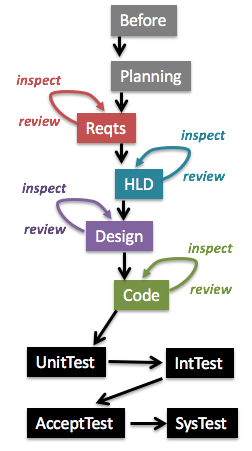
\includegraphics[width=1.6in]{wfall.png}  
\end{center}
\caption{Phases of our data.
Abbreviations: 
{\em Before}= before development; 
{\em Reqts}	  = requirements; 
{\em HLD}	  = high-level design; 
{\em IntTest} = Integration testing (with code from others); 
{\em SysTest} = system test (e.g. load stress tests); 
{\em AcceptTest}  = acceptance testing (with users); 
{\em review}        = private activity; 
{\em inspect}        = group activity.}
\label{fig:waterfall}
\end{figure}

The \textit{development phases} against which plan items are logged in the data are shown in \fig{waterfall}.
Although the representation suggests a waterfall model, the SEI experience is that the projects follow a spiral approach or perform the work in iterative and/or incremental development cycles. The phases are thus the logical stages through which each increment must progress during development.

One special feature of  \fig{waterfall} is the {\em before} phase, in which the TSP team assures that management has clearly identified cost, schedule, and scope goals appropriate to the upcoming development activities, often including a conceptual model~\cite{Humphrey:2005}. For example an architecture team must have sufficient requirements to reason about, prototype, and specify an architecture~\cite{Bachmann13} while a coding only team within a larger project would have more precisely defined requirements and high level design.
 
%Within a project increment, multiple features or components may be developed and incremented. TSP is compatible %with agile and encourages iterative and incremental development. Nonetheless, the specific strategy and cycle %duration is a project decision. TSP does, however, strongly encourage 1) constructing units of sufficient size that %%measurement is practicable, and 2) separating the construction from appraisal and test activities. This %effectively highlights the separation of construction from rework activities and aids the apportionment of defects %to those found in appraisal activities (reviews and inspections) and those found through failure (test). The %distinct construction activities (requirements, high and detailed design, and code) were chosen to help teams %analyze the effectiveness and efficiency of their practices through analysis of the defect phase origin, type, fix %effort, and phase of discovery. 

Note that, in Figure~\ref{fig:waterfall}, several  phases in which the product is created have sub-phases of {\em review} and {\em inspect} to remove defects. As discussed in \S\ref{sect:tsp}, individuals perform personal reviews of their work products prior to the peer review (which TSP calls the inspection). Testing activities are divided as follows. Developers perform unit test prior to code complete.  After code complete a standard phase is integration, which combines program units into a workable system ready for system test. Integration,  system test, and acceptance test are often performed by another group. 


    
 
\subsection{Data Integrity}
\label{sect:data_integrity}

A common property of real-world data sets is the presence
of noisy entries (superfluous  or spurious data). 
The level of noise can be quite high. For example, as reported
in \cite{shepperd12}, around
10\% to 30\%
of the records in the NASA MDP defect data sets are
affected by noise. 

One reason to use the SEI data for the analysis of this paper is its remarkably low level of noise.
Nichols et al.~\cite{shirai14}  report that
the noise levels in the SEI TSP data are smaller than those seen
in other data sets. They found in the SEI TSP data that:\bi 
\item
4\% of the data was incorrect (e.g. nulls, illegal formats);
\item  2\% of the data has inconsistencies such as timestamps
where the stop time was before the start time;
\item 3\% of the data contained values that were not credible
such as tasks listed in one day that took more than six hours for a single developer.
\ei 
One explanation for this low level of noise is the TSP process.
One the guiding principles of TSP was that  people performing the work are  responsible for planning and tracking the work. That is,  all the data collected here was entered
by local developers, who use the data for planning and tracking their projects. This data was then checked by local coaches before being sent to the SEI
databases. While coaches are certified by demonstrating competent use of the TSP process with the artifacts and data,  project success or performance is not a criterion. 
The use of certified local coaches within each project increases the integrity of our data.


 

\subsection{Project Descriptive Characteristics}
\label{sect:data_character}

%\todo{should we add a citation to Petersen and a few more words on context.}
In this section we provide some descriptive statistics and discuss the of the projects from which this data was drawn and summarize some additional contextual information. The project contexts describe the conditions under which these measures were obtained, help determine relevance of the results, and may guide future data analysis with segmentation. Key attributes of the context include the business and application domains, product size, project duration,  work flows, team size, team management,  development and integration approaches, organization size, location or distribution, certifications, developer experience, programming languages and tools used. 

We are unable at this time to provide all individual context data for each of the projects for several reasons. While the development data was recorded in tools and submitted in a structured form, context data was collected in less structured project questionnaires, site questionnaires, team member surveys, launch presentations and reports, post mortem presentations and reports. This data has not yet been mined from the submissions 1) because of the cost and effort required, 2) we are obligated to avoid providing any data that can identify projects (that is, the data must remain anonymous), and 3) the unstructured data is not always  complete  submitted.   Gathering more projects will make it easier to anonymize the data and overcome missing data problems. Interest in the data sets by the community may encourage our sponsor to fund additional data mining.  Nonetheless, much context is available from the project data  and we provide some additional context not included within the fact sheets. 
 
 The projects included come from 45 unique organizations from 6 countries. \fig{nationality} shows the country of origin and application domains for the projects.  \fig{number of projects per organization} shows the number of projects from each organization. 
 
The most common countries of origin are the US and Mexico. Not apparent in this display is that the US companies tend to be fewer and larger with many projects while the Mexican companies are more likely to have one to several projects. Several companies, typically larger companies, are international with development teams in the US and either France or China. 

The most common project application domains are banking, consumer applications, engineering design tools, and medical devices.   
The data for programming languages is incomplete, with most projects using more than one language, but few reporting  programming language by component or size.  The list of languages includes ABAP, ADA, Alpha, C, C++, C\#, ASP.net, Delphi, Gauss, Genexus, Hotware, HTML, Java, JavaScript, PHP, PLSQL, Ruby, SQL, and Visual Basic. 
 

 The specific process work flows and practices are developed by the development team personnel who have received specific training on defining work processes as part of their Personal Software Process training. The process data was collected by the team members to self-manage their personal and team work. Them members also exhibited self-management behavior by estimating planning and scheduling the work tasks. 

While the processes and work flows among these projects can vary, the logical order is described section \ref{development_phase} is followed. Development tasks such as requirements development, design, or code, are typically followed by an appraisal phase such as personal review or inspection. Effort and effectiveness of these activities vary among projects and developers.


\begin{figure}[ht]
\scriptsize
\centering
\begin{tabular}{cc}
\begin{tabular}[t]{lr}
Country      & \% of projects \\\hline
China        & 1.0 \%            \\
France       & 10.0 \%           \\
Mexico       & 41.0 \%           \\
South Africa & 4.0 \%            \\
UK           & 1.5 \%          \\
US           & 42.5 \%        
\end{tabular}
&
\begin{tabular}[t]{lr}
Application Domain         & count \\\hline
Aviation                   & 19    \\
Banking                    & 23    \\
Business intelligence      & 19    \\
Construction Support tools & 3     \\
Consumer applications      & 24    \\
Custom Applications        & 1     \\
Embedded systems           & 2     \\
Engineering Design Tools   & 21    \\
Geography and Mapping      & 2     \\
Government                 & 5     \\
Human Resources Management & 3     \\
Information Technology     & 1     \\
Manufacturing              & 3     \\
Medical Devices            & 15    \\
Other                      & 2     \\
Payroll services           & 1     \\
Solutions Integration      & 1     \\
Web applications           & 13    \\
Wholesale or retail trade  & 9    
\end{tabular}
\end{tabular}
\caption{Project nationality and application domain}
\label{fig:nationality}
\end{figure}

 
\begin{figure}[!t] 
\begin{center}
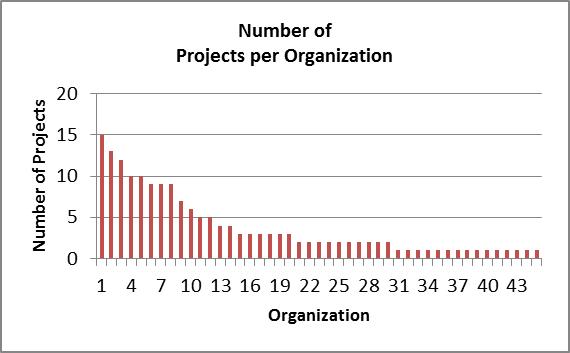
\includegraphics[height=1.5in]{number_of_projects_per_org.png}
\end{center} 
\caption{Number of projects per development organization.}
\label{fig:number of projects per organization}
\end{figure}


 
 
 \begin{figure}[ht]
\scriptsize
\centering
\begin{tabular}{llr} 
 Begin Phase &  Final Phase & Count  \\\hline
  Requirements      & Unit Test                   & 12  \\ 
  Requirements      & Build and Integration Test  & 19  \\ 
  Requirements      & System Test                 & 36  \\ 
  High Level Design & Unit Test                   & 3  \\ 
  High Level Design & Build and Integration Test  & 10  \\ 
  High Level Design & System Test                 & 9  \\ 
  Detailed Level Design & Unit Test                   & 18  \\ 
  Detailed Level Design & Build and Integration Test  & 24  \\ 
  Detailed Level Design & System Test                 & 17  \\ 
\end{tabular}
\caption{Earliest and latest process phases used by the projects}
\label{fig:earliest-and-least-process-phases}
\end{figure}
 


 
 The project schedule, cost, and scope  are characterized by calendar duration, development team size project, and product size (measured in added and modified lines of code and number of components).  These data are all available from the project fact sheets for each project. Summary statistics and the year of project initiation are displayed in Figure~\ref{fig:Project-descriptive-stats}. From this table we can make some observations about the range of project characteristics .
 
 \begin{figure}[ht]
\scriptsize
\centering
\begin{tabular}{lrrrrrrrl}
                                                                   & N   & Min & Q1   & Median & Q3    & Max   & Mean   &  Distribution \\\hline
Team size                                                          & 171 & 1   & 4    & 6      & 10    & 36    &  7.8    &  
\includegraphics[width=15mm]{team_size.png} \\ 
Duration {[}days{]}                                                & 171 & 7   & 33   & 61     & 118   & 1918  & 107    & 
\includegraphics[width=15mm]{duration.png} \\
Added \& Modified LOC                                                 & 117 & 2   & 1125 & 4201   & 13092 & 88394 & 10259  & 
\includegraphics[width=15mm]{LOC.png} \\
Components                                                         & 171 & 8   & 26   & 49     & 107   & 4170  & 116.2  & 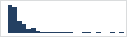
\includegraphics[width=15mm]{components.png} \\
Year                                                               & 171 &     & 2011 & 2012   & 2013  & 2014  & 2011.9 & 
\includegraphics[width=15mm]{year.png}
\end{tabular}

\caption{Project summary description}
\label{fig:Project-descriptive-stats}
\end{figure}
 
 
 Of the 171 projects in the sample, only 117 collected size data in lines of code, however all projects tracked effort and  the component counts with applied effort are provided. Other data is complete for all 171 projects. The projects were mostly of short duration and small to medium size. The median project began in 2012 lasted 61 days, produced 4200 Lines of Code, 49 components (modules or features). Duration ranged from 7 to 1918 days. Size ranged from minimal (this may represent a short maintenance project) to 88394. The earliest project was in 2006 and the most recent in 2014. 
 
How many of these teams could be classified as "agile" is not clear because actual practices in the agile world can vary. We did not ask teams to self-identify, however we offer the following observations regarding characteristics commonly associated with agile behavior. 
\begin{itemize}
    \item all teams were self managed, defining work flows, practices, and schedules
    \item teams meet at least weekly to evaluate progress and replan
    \item most teams were small with a median size of 6 and a mean of 7.8. only 25\% of the teams were larger than 10 with a long tail on the distribution
    \item the median project lasted only 60 days, suggesting limited scope for each integration
\end{itemize}
  


\begin{figure}[!t] 
\vspace{0.5cm}
\begin{center}
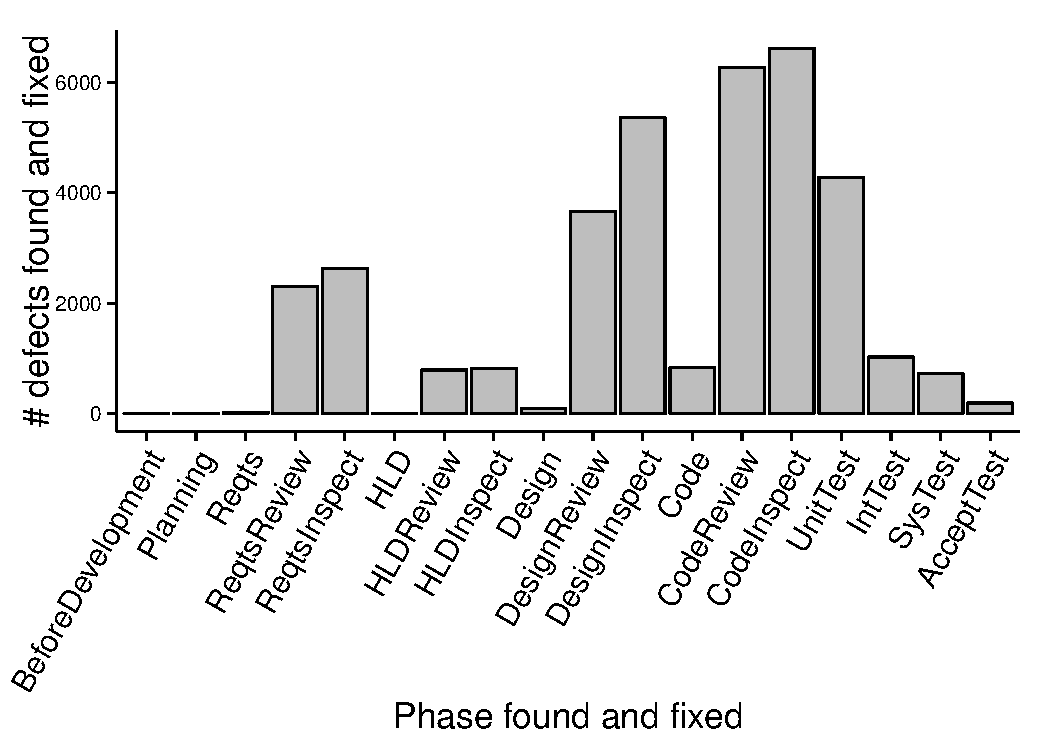
\includegraphics[height=2.5in]{fix-phase-dist.pdf}
\end{center} 
\caption{Distribution of defects found and fixed by phase.}
\label{fig:fix-phase-dist}
\end{figure}





\subsection{Statistical Analysis}\label{sect:stats}
    
    In the following presentation of our results, three statistical methods were used to test for the delayed
    issue effect: the Scott-Knott ranker;   bootstrap sampling (to test for statistical significantly
    different results); and an effect size test (to reject any significant differences that are trivially small).
    
    The Scott-Knott ranker 
      was   recommended  by  Mittas and Angelis in a
    recent TSE'13 article~\cite{mittas13} and by Ghotra et al. in a recent
    ICSE'15 article~\cite{ghotra2015icse}
    Scott-Knott is a 
    top-down clustering approach used to rank different treatments. If that 
    clustering finds an ``interesting division'' of the data, then some 
    statistical test is applied to the two divisions to check if they are 
    statistically significant different. If so, Scott-Knott considers recurses into both 
    halves.
    Before Scott-Knot recurses,  however,  it apples some  statistical hypothesis test $H$ to check
    if $m,n$ are significantly different. 
    
    To operationalize ``interesting'', Scott-Knott seeks the division of 
    of $l$ treatments into subsets of size $m,n$ of sizes $ls,ms,ns$ and median values
    $l.\mu, m.\mu, n.\mu$ (respectively) in order to maximize
 $\frac{ms}{ls}abs(m.\mu - l.\mu)^2 + \frac{ns}{ls}abs(n.\mu - l.\mu)^2$.
   
   To operationalize $H$, we use both  bootstrap sampling  and the A12 effect size test.
   In other 
    words, we divide the data if \textit{both} bootstrap sampling and effect 
    size test agree that a division is statistically significant (with a 
    confidence of 99\%) and not a small effect ($A12 \ge 0.6$).
    For a justification of the use of non-parametric bootstrapping, see Efron 
    \& Tibshirani~\cite[p220-223]{efron93}. For a justification of the use of 
    effect size tests see Shepperd and MacDonell~\cite{shepperd12a}; 
    Kampenes~\cite{kampenes07}; and Kocaguenli et 
    al.~\cite{Kocaguneli2013:ep}. These researchers warn that even if a 
    hypothesis test declares two populations to be ``significantly'' 
    different, then that result is misleading if the ``effect size'' is very 
    small. Hence, to assess the performance differences we first must rule out 
    small effects using A12, a test   recently endorsed by Arcuri and 
    Briand at ICSE'11~\cite{arcuri11}.
  
    
    To  apply Scott-Knott, we divided data into the phases $P_0$ where issues are introduced. Next, for each division, we separated all the issues that were removed at different subsequent issues $P_r \in \{P_1,P_2,..\}$.
    For each pair $P_0,P_r$, we build one treatment containing the  issue resolution times for     issues raises in $P_0$ and resolved in $P_r$. These treatments
    were then ranked by Scott-Knott. 
     
   
    


\begin{figure} 
% \renewcommand{\baselinestretch}{0.8}
% \small
\begin{center}

%\resizebox{\columnwidth}{!}{
\scriptsize
\begin{tabular}{c|lr|rr|rl}
& \multicolumn{2}{c|}{ } & \multicolumn{2}{c|}{Percentiles} & \multicolumn{2}{c}{~ } \\ 
  & \multicolumn{2}{c|}{ } & \multicolumn{2}{c|}{(units = } & \multicolumn{2}{c}{Growth with respect to earliest phase  } \\ 
   & \multicolumn{2}{c|}{Phase} & \multicolumn{2}{c|}{  minutes)} & \multicolumn{2}{c}{(unitless  ratios of two time values) } \\\hline


  rank & injected & removed & 50th &   IQR & \multicolumn{2}{c}{50th percentile growth}  \\ 
\hline

\multicolumn{7}{c}{~}  \\
1 &  Before   
      &   DesignInspect   & 10 &  14 & 1.00 & \textcolor{black}{\rule{10mm}{2mm}}  \\
1 &   &   CodeReview      & 8 &  14 & 0.80 & \textcolor{black}{\rule{8mm}{2mm}}  \\
1 &   &   CodeInspect     & 10 &  16 & 1.00 & \textcolor{black}{\rule{10mm}{2mm}}  \\
1 &   &   UnitTest        & 12 &   21 & 1.20 & \textcolor{black}{\rule{12mm}{2mm}}  \\
1 &   &   IntTest         & 15 &   31 & 1.50 & \textcolor{black}{\rule{15mm}{2mm}}  \\
1 &   &   SysTest         & 11 &   22 & 1.10 & \textcolor{black}{\rule{12mm}{2mm}}  \\  
\hline\multicolumn{7}{c}{~}  \\
1 &  Planning     &   ReqtsReview     & 8 &  14 & 1.00 & \textcolor{black}{\rule{10mm}{2mm}}  \\
1 &               &   DesignInspect   & 11 &  13 & 1.38 & \textcolor{black}{\rule{13mm}{2mm}} \\
2 &               &   UnitTest        & 24 &   25 & 3.00 & \textcolor{black}{\rule{30mm}{2mm}} \\
\hline\multicolumn{7}{c}{~}  \\
1 &  Reqts   &   ReqtsReview     & 13 &  20 & 1.00 & \textcolor{black}{\rule{10mm}{2mm}} \\
1 &          &   ReqtsInspect    & 12 &   18 & 0.92 & \textcolor{black}{\rule{9mm}{2mm}}  \\
1 &          &   DesignReview    & 10 &   14 & 0.77 & \textcolor{black}{\rule{7mm}{2mm}} \\
1 &          &   DesignInspect   & 9 &   15 & 0.69 & \textcolor{black}{\rule{6mm}{2mm}}   \\
1 &          &   CodeInspect     & 13 &  24 & 1.00 & \textcolor{black}{\rule{10mm}{2mm}} \\
1 &          &   UnitTest        & 10 &  17 & 0.77 & \textcolor{black}{\rule{7mm}{2mm}}  \\
1 &          &   IntTest         & 33 &   42 & 2.54 & \textcolor{black}{\rule{25mm}{2mm}}  \\
1 &          &   SysTest         & 24 &  108 & 1.85 & \textcolor{black}{\rule{18mm}{2mm}}  \\
\hline\multicolumn{7}{c}{~}  \\
1 & Design   &   DesignReview    & 11 &   16 & 1.00 & \textcolor{black}{\rule{10mm}{2mm}}  \\
1 &   &   DesignInspect   & 8 &   12 & 0.73 & \textcolor{black}{\rule{7mm}{2mm}}  \\
1 &   &   CodeReview      & 10 &   18 & 0.91 & \textcolor{black}{\rule{9mm}{2mm}}  \\
1 &   &   CodeInspect     & 9 &  14 & 0.82 & \textcolor{black}{\rule{8mm}{2mm}}  \\
1 &   &   UnitTest        & 11 &   18 & 1.00 & \textcolor{black}{\rule{10mm}{2mm}}  \\
1 &   &   IntTest         & 17 &   31 & 1.55 & \textcolor{black}{\rule{15mm}{2mm}}  \\
1 &   &   AcceptTest      & 14 &   19 & 1.27 & \textcolor{black}{\rule{12mm}{2mm}}  \\
1 &   &   SysTest         & 13 &   18 & 1.18 & \textcolor{black}{\rule{12mm}{2mm}}  \\
\hline\multicolumn{7}{c}{~}  \\
1 &  Code   &   CodeReview    & 10 &  16 & 1.00 & \textcolor{black}{\rule{10mm}{2mm}}  \\
1 &    &   CodeInspect   & 10 &   15 & 1.00 & \textcolor{black}{\rule{10mm}{2mm}}  \\
1 &   &   UnitTest      & 12 &   20 & 1.20 & \textcolor{black}{\rule{12mm}{2mm}}  \\
1 &    &   IntTest       & 14 &   25 & 1.40 & \textcolor{black}{\rule{14mm}{2mm}}  \\
1 &    &   AcceptTest    & 16 &   25 & 1.60 & \textcolor{black}{\rule{16mm}{2mm}}  \\
1 &   &   SysTest       & 13 &   20 & 1.30 & \textcolor{black}{\rule{13mm}{2mm}}  \\

\end{tabular}
%}
%
% \begin{tabular}{l@{~~~}r|r@{~}r|r@{~}lr@{~}l} 
% \renewcommand{\baselinestretch}{0.5}
% \multicolumn{2}{l|}{Phase}&\multicolumn{2}{c|}{Percentile}&\multicolumn{4}{c}{Ratio w.r.t. to phase where issue was injected}\\\hline
%  injected&removed&50th&95th&\multicolumn{2}{c|}{50th}&\multicolumn{2}{c}{95th}\\\hline
% \\
% Before&DesignInspect&30&97&1&\rule{10mm}{2mm}&1&\textcolor{red}{\rulree{10mm}{2mm}} \\
% &CodeReview&28&94&0.93&\rule{9mm}{2mm}&0.96&\textcolor{red}{\rule{10mm}{2mm}} \\
% &CodeInspect&45&154&1.5&\rule{15mm}{2mm}&1.58&\textcolor{red}{\rule{16mm}{2mm}} \\
% &UnitTest&77&187&2.56&\rule{26mm}{2mm}&1.92&\textcolor{red}{\rule{19mm}{2mm}} \\
% &IntTest&65&424&2.16&\rule{22mm}{2mm}&4.37&\textcolor{red}{\rule{35mm}{2mm}} \\
% &SysTest&56&164&1.86&\rule{19mm}{2mm}&1.69&\textcolor{red}{\rule{17mm}{2mm}} \\\hline\\
% Planning&ReqtsReview&35&99&1&\rule{10mm}{2mm}&1&\textcolor{red}{\rule{10mm}{2mm}} \\
% &DesignInspect&24&81&0.68&\rule{7mm}{2mm}&0.81&\textcolor{red}{\rule{8mm}{2mm}} \\
% &UnitTest&33&238&0.94&\rule{9mm}{2mm}&2.4&\textcolor{red}{\rule{24mm}{2mm}} \\\hline\\
% Reqts&ReqtsReview&92&240&1&\rule{10mm}{2mm}&1&\textcolor{red}{\rule{10mm}{2mm}} \\
% &ReqtsInspect&93&243&1.01&\rule{10mm}{2mm}&1.01&\textcolor{red}{\rule{10mm}{2mm}} \\
% &DesignReview&33&119&0.35&\rule{4mm}{2mm}&0.49&\textcolor{red}{\rule{5mm}{2mm}} \\
% &DesignInspect&49&137&0.53&\rule{5mm}{2mm}&0.57&\textcolor{red}{\rule{6mm}{2mm}} \\
% &CodeInspect&38&156&0.41&\rule{4mm}{2mm}&0.65&\textcolor{red}{\rule{7mm}{2mm}} \\
% &UnitTest&49&180&0.53&\rule{5mm}{2mm}&0.75&\textcolor{red}{\rule{8mm}{2mm}} \\
% &IntTest&67&300&0.72&\rule{7mm}{2mm}&1.25&\textcolor{red}{\rule{13mm}{2mm}} \\
% &SysTest&122&459&1.32&\rule{13mm}{2mm}&1.91&\textcolor{red}{\rule{19mm}{2mm}} \\\hline\\
% Design&DesignReview&103&331&1&\rule{10mm}{2mm}&1&\textcolor{red}{\rule{10mm}{2mm}} \\
% &DesignInspect&101&272&0.98&\rule{10mm}{2mm}&0.82&\textcolor{red}{\rule{8mm}{2mm}} \\
% &CodeReview&66&215&0.64&\rule{6mm}{2mm}&0.64&\textcolor{red}{\rule{6mm}{2mm}} \\
% &CodeInspect&79&259&0.76&\rule{8mm}{2mm}&0.78&\textcolor{red}{\rule{8mm}{2mm}} \\
% &UnitTest&119&383&1.15&\rule{12mm}{2mm}&1.15&\textcolor{red}{\rule{12mm}{2mm}} \\
% &IntTest&88&337&0.85&\rule{9mm}{2mm}&1.01&\textcolor{red}{\rule{10mm}{2mm}} \\
% &SysTest&80&336&0.77&\rule{8mm}{2mm}&1.01&\textcolor{red}{\rule{10mm}{2mm}} \\
% &AcceptTest&45&120&0.43&\rule{4mm}{2mm}&0.36&\textcolor{red}{\rule{4mm}{2mm}} \\\hline\\
% Code&CodeInspect&113&337&1&\rule{10mm}{2mm}&1&\textcolor{red}{\rule{10mm}{2mm}} \\
% &CodeReview&115&300&1.01&\rule{10mm}{2mm}&0.89&\textcolor{red}{\rule{9mm}{2mm}} \\
% &UnitTest&133&434&1.17&\rule{12mm}{2mm}&1.28&\textcolor{red}{\rule{13mm}{2mm}} \\
% &IntTest&125&473&1.1&\rule{11mm}{2mm}&1.4&\textcolor{red}{\rule{14mm}{2mm}} \\
% &SysTest&95&383&0.84&\rule{8mm}{2mm}&1.13&\textcolor{red}{\rule{11mm}{2mm}} \\
% &AcceptTest&65&360&0.57&\rule{6mm}{2mm}&1.06&\textcolor{red}{\rule{11mm}{2mm}} \\

% \end{tabular}

\end{center}
\caption{Median times to resolve issues seen in the SEI TSP data. The main effect here is that there is no clear exponential growth in the time to resolve issues as issues are injected in some phase $P_0$ then resolved in some subsequent issue $P_r$.
Shown where are the 50th percentiles of issue resolution times for issues injected in phase $P_O$ and resolved in phase $P_r$ (these values are calculated
by sorting all resolution time, then reporting the middle values of that sort)
The ``IQR'' column shows the ``inter-quartile range''; i.e. the range of values representing the 75th - 25th percentile range
The left-hand-side ``rank'' column shows the result of the Scott-Knott ranking procedure described in \tion{stats}. Note that
most treatments achieved the same ranks i.e. they were found to be insignificantly different  from each other (the one exception is the Planning:UnitTest results 
where UnitTests were ranked 2).
The right-hand-side bars
illustrate shows the releative sizes of the increases for the  50th (median)   percentile values. These increases are calculated with respect to the first value in each section ``Before, Planning, Reqts. Design, Code''.
These right-hand-side bars are unitless since they are ratios. For example,
on the last line, issues injected during coding and fixed in SysTest take 13 minutes (median) to resolve. This is 130\% more than the 10 minutes (median) required
to resolve coding issues during CodeReview. The right-hand-side bar visually represents that 130\%.}
\label{fig:raw}
\end{figure}
 
 
\subsection{Observations from 171 Projects}\label{sect:171projects}

The distribution by phase in which defects were discovered (that is both found and fixed) in our data is shown in Figure~\ref{fig:fix-phase-dist}. Defects are counted only if they they escape the introduction phase unless a bad fix introduces a new defect.  These secondary defects occur almost exclusively in test and very rarely in an inspection. 
A high percentage of defects (44\%) were found and fixed in the early phases, i.e., prior to coding. This distribution is similar to that observed for other projects that emphasized investment in software engineering quality assurance practices. For example, Jones and Bonsignour report 52\% of pretest defects removed before entering implementation, for large projects that focus on upfront defect removal techniques \cite{jones12}. NASA robotics projects had a slightly higher percentage (58\%) of defects removed before implementation began, although these had invested in independent verification and validation on top of other forms of defect removal \cite{me08a}.  

\fig{raw} shows the  50th  percentile
of the time spent resolving issues
(note that, in TSP, when developers see issues, they enter {\em review} or 
{\em inspect} or {\em test}
until that issue is retired).
These values include all the time required  to (a)~collect data and realize there is an error;
(b)~prepare a fix;  and (c)~apply some validation
procedure to check the fix (e.g. discuss it with a colleague or execute some tests).


In \fig{raw}, the data is split out according to issues that were fixed in phase $P_r$ after
being introduced in phase $P_0$. The data is sub-divided into tables according to $P_0$;
i.e. according to {\em before, planning, requirements, design} or {\em  code}. 
To ensure the representativeness of each line, we display examples
where there exists at least $N\ge 30$ examples\footnote{We selected 30
for this threshold via the central limit theorem~\cite{maxwelldata}.} of issues {\em injected} in phase $P_0$ then
removed in phase $P_r$.
The right hand side bars of that figure
illustrate how these resolutions increase (expressed as ratios of resolution time in the phase where they were first injected).


The two key features of \fig{raw} are:
\be
\item Nowhere in
these results do we see the kind of very large increases reported in the papers
documenting DIE. For example, consider the ratio of the issue resolution time
between {\em Before/DesignInspect} and {\em Before/SysTest} result. That ratio is 1.11 which is far smaller
than the scale ups seen in \fig{b81}.  
\item
Nearly all the supposed increases seen in \fig{raw} are insignificantly different
to the other treatments.  The left hand column of \fig{raw} shows the results of the Scott-Knott statistical tests. Note that nearly all
the treatments have the same rank (``1''); i.e. usually there is no statistically significant difference in the 
time to resolve issues. The only exception here is Planning:UnitTest which is ranked ``2'' but even here, the scale up is merely
a factor of 3, and not the exponential increase promised by classic reports of the delayed issue effect.
\ee
One possible explanation for the lack of a DIE effect is that we are looking
broadly at the entire data set but not at specific stratifications. To address that concern,
we spent some time reproducing \fig{raw} for various subsets of our data.
That proved to be an unfruitful-- no stratification was found that 
contained an exponential expansion in the time to fix issues. The reason for this was  the small size
of those stratifications  exacerbated the large IQR's seen in this data\footnote{Recall that in a sorted list of numbers,
the inter-quartile range, or IQR, is difference between the 
  75th to 25th percentile value.}.
Our 171 projects   stratifies into subsets of varying sizes. Sorting those sizes, we get a list
comprising of 17,12 then numerous much smaller stratifications.  Reasoning over such small samples
is problematic in the general case and, in the case of our data, it is ever more problematic due to
the large IQRs of the data
(to see these large IQRs,  please consider the 50th and IQR columns of Figure~\ref{fig:raw} where  most of our IQRs were larger than tan the 50th percentile; i.e. software
data exhibits large variances-- where are exacerbated by the smaller samples seen in the stratifications).
Our conclusion from exploring the stratification's is that, given the currently available data, we cannot check
for a DIE effect in subsets of this data.


Before moving on, we comment on some of the counter-intuitive
results in \fig{raw}. Consider, for example, the ``Reqts'' results were
the time required to fix issues actually tends to {\em decrease} the longer they are left in the system. In terms of explaining this result, the key thing is the left-hand-side statistically ranking: all these treatments were found to be statistically indistinguishable. In such a set of treatments, the observed
difference may {\em not} be a causal effect; rather, it may just
be the result of  random noise.

%In summary:
%\bi
%\item
%\item
%But there is no trace of that  effect   in hundreds of software projects built  since 2006.
%\ei
%For illustrative purposes, the relative cost to fix errors per lifecycle phase in the TSP project data is overlayed with Boehm's cost curve~\cite{Boehm81} as well as the CCPDS-R case study~\cite{Royce98} in \fig{cost-to-fix-tsp}. Cost-to-fix for TSP is total time spent in each review, inspection, or test-related phase / \# of defects found in phase (reported in \fig{raw}). It is clear to see that the trend is relatively flat, closer to the pattern exhibited by the Royce case study (which also focused on early defect removal) than the exponential growth curve.
 


%\begin{figure}[!t] 
%%\vspace{-1cm}
%\hspace{-0.35in}
%\begin{center}
%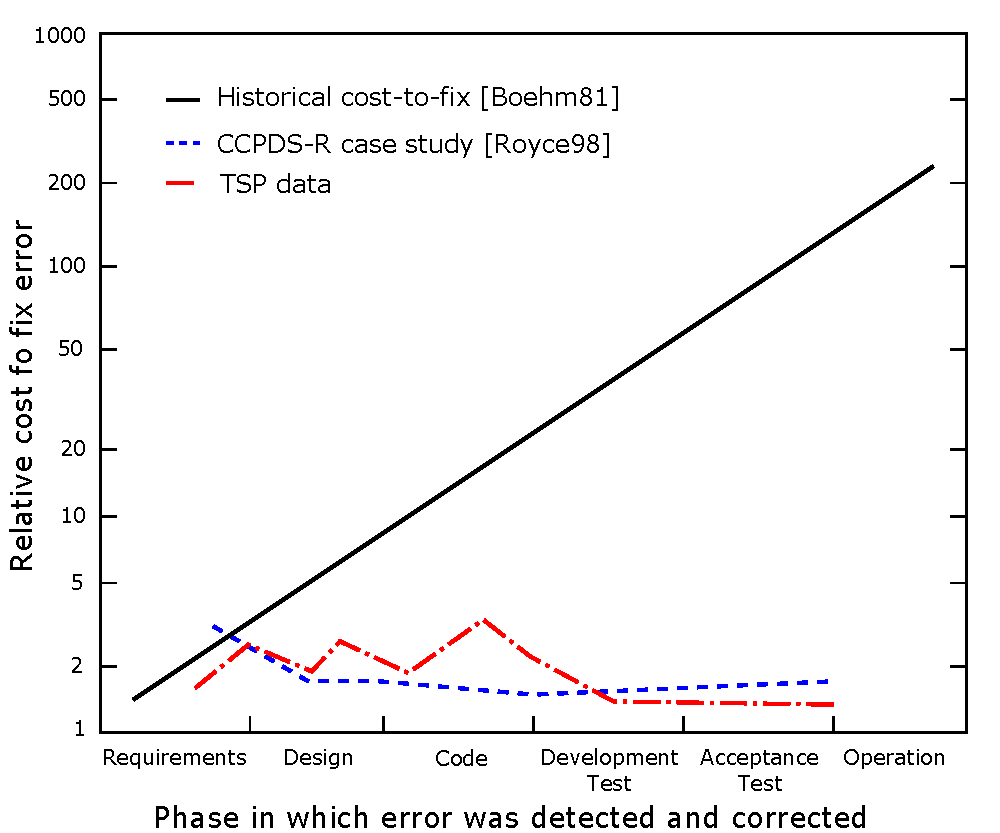
\includegraphics[width=3in]{img/boehm-overlay.pdf}
 %\end{center}
% ~\\~\\
%~\\~\\~\\
 
 %\caption{Cost-to-fix curve from \protect\fig{cost-to-fix} 
 %overlayed with case study from~\cite{Royce98} and TSP data. Scale is relative to the phase with the lowest %c%ost to fix. }\label{fig:cost-to-fix-tsp}
% \end{figure}
 
%\begin{table}[ht]
%\renewcommand{\baselinestretch}{0.7}
% \scriptsize
%\centering
%\begin{tabular}{ll|ll}
%  Phase num & Name & \# defects & percentage \\ 
%  \hline
%1 & BeforeDevelopment &   0 & 0.00 \\ 
%  2 & Planning &   4 & 0.00 \\ 
%  3 & Reqts &  25 & 0.10 \\ 
%  4 & ReqtsReview & 2304 & 6.50 \\ 
%  5 & ReqtsInspect & 2630 & 7.40 \\ 
%  6 & HLD &   0 & 0.00 \\ 
%  7 & HLDReview & 790 & 2.20 \\ 
%  8 & HLDInspect & 818 & 2.30 \\ 
%  9 & Design &  94 & 0.30 \\ 
%  10 & DesignReview & 3668 & 10.30 \\ 
%  11 & DesignInspect & 5365 & 15.00 \\ 
%  12 & Code & 833 & 2.30 \\ 
%  13 & CodeReview & 6276 & 17.60 \\ 
%  14 & CodeInspect & 6623 & 18.60 \\ 
%  15 & UnitTest & 4283 & 12.00 \\ 
%  16 & IntTest & 1024 & 2.90 \\ 
%  17 & SysTest & 730 & 2.00 \\ 
%  18 & AcceptTest & 189 & 0.50 \\ 
% \end{tabular}
%\caption{Defects found per phase} 
%\label{fig:defect_per_phase}
%\end{table}



%\begin{figure}[!ht]
%
% \renewcommand{\baselinestretch}{0.7}
% \scriptsize
%\begin{center}
%\begin{tabular}{r|rr|rl}
%Phase & samples & total time&\multicolumn{2}{l}{Total time w.r.t. first phase}\\\hline
%~\\
%Planning&229&12625&1.00&*\\
%~\\
%Reqts&590&24182&1.91&**\\
%ReqtsInspect&2533&92723&7.34&********\\
%ReqtsReview&1762&67471&5.34&******\\
%~\\
%HLD&78&6856&0.54&*\\
%HLDReview&472&12821&1.01&**\\
%HLDInspect&1366&35291&2.79&***\\
%~\\
%Design&620&21573&1.70&**\\
%DesignInspect&8373&229937&18.21&*******************\\
%DesignReview&3043&92823&7.35&********\\
%~\\
%Code&3029&220058&17.43&******************\\
%CodeReview&4774&163091&12.91&*************\\
%CodeInspect&11406&334442&26.49&***************************\\
%~\\
%UnitTest&9177&352245&2.790&****************************\\
%IntTest&2761&160559&12.71&*************\\
%SysTest&2059&105796&8.37&*********\\
%AcceptTest&1045&42717&0.338&****\\
%\end{tabular}
%\end{center}
%\caption{Times per phase (minutes).}
%\label{fig:fix-time-per-phase}
%\end{figure}



%we calculate phase delay as simply the number of project phases (the set used in our data set is shown in %\fig{waterfall}) during which the defect existed in the system, i.e. the ordinal rank of removal phase minus the %ordinal rank of injection phase. Sub-phases (such as review and inspection) are included in this calculation.
%


 
 %\begin{figure}[!t]
%\%renewcommand{\baselinestretch}{0.7}
%\scriptsize
%\begin{center}
%\begin{tabular}{l@{~~}|l@{~}|r@{~}|r@{~}r@{~}|r@{~}l}
%%           \multicolumn{2}{c}{~}                 &  &\multicolumn{2}{c|}{median}\\
 % Injection&   Removal& $n$ & initial & now & \multicolumn{2}{l}{Scale up, w.r.t. initial}
%\\\hline

BeforeDevelopment&Code.dat&57&1&\rule{2mm}{2mm} \\
BeforeDevelopment&CodeInspect.dat&72&0.3&\rule{0mm}{2mm} \\
BeforeDevelopment&Test.dat&165&1.1&\rule{2mm}{2mm} \\
BeforeDevelopment&IntTest.dat&50&1.3&\rule{2mm}{2mm} \\
BeforeDevelopment&SysTest.dat&42&1.8&\rule{2mm}{2mm} \\
\\\hline

Planning&Planning.dat&66&1&\rule{2mm}{2mm} \\
Planning&ReqtsReview.dat&41&0.8&\rule{0mm}{2mm} \\
\\\hline

Reqts&Reqts.dat&23&1&\rule{2mm}{2mm} \\
Reqts&ReqtsReview.dat&245&13&\rule{26mm}{2mm} \\
Reqts&ReqtsInspect.dat&289&16&\rule{32mm}{2mm} \\
Reqts&Design.dat&32&21&\rule{42mm}{2mm} \\
Reqts&DesignInspect.dat&49&7&\rule{14mm}{2mm} \\
\\\hline
 

HLD&HLDReview.dat&94&1&\rule{2mm}{2mm} \\
HLD&HLDInspect.dat&133&1.6&\rule{2mm}{2mm} \\
HLD&Design.dat&33&1&\rule{2mm}{2mm} \\
\\\hline

Design&Design.dat&37&1&\rule{2mm}{2mm} \\
Design&DesignInspect.dat&455&6&\rule{12mm}{2mm} \\
Design&Code.dat&218&3.5&\rule{6mm}{2mm} \\
Design&CodeInspect.dat&166&2.7&\rule{4mm}{2mm} \\
Design&Test.dat&542&7.7&\rule{14mm}{2mm} \\
Design&IntTest.dat&67&3.7&\rule{6mm}{2mm} \\
Design&SysTest.dat&92&6.3&\rule{12mm}{2mm} \\
\\\hline

DesignInspect&DesignInspect.dat&53&1&\rule{2mm}{2mm} \\
DesignInspect&Code.dat&38&0.75&\rule{0mm}{2mm} \\
\\\hline

Code&Code.dat&126&1&\rule{2mm}{2mm} \\
Code&CodeInspect.dat&459&2&\rule{4mm}{2mm} \\
Code&Test.dat&461&2.16667&\rule{4mm}{2mm} \\
Code&IntTest.dat&348&2.16667&\rule{4mm}{2mm} \\
Code&SysTest.dat&230&1.5&\rule{2mm}{2mm} \\
Code&AcceptTest.dat&71&0.916667&\rule{0mm}{2mm} \\
\\\hline

CodeInspect&CodeInspect.dat&64&1&\rule{2mm}{2mm} \\
CodeInspect&Test.dat&57&1.25&\rule{2mm}{2mm} \\
\\\hline

Test&Test.dat&110&1&\rule{2mm}{2mm} \\
Test&QualTest.dat&66&0.4&\rule{0mm}{2mm} \\
\\\hline

IntTest&QualTest.dat&32&1&\rule{2mm}{2mm} \\
IntTest&IntTest.dat&36&5.5&\rule{10mm}{2mm} \\
IntTest&SysTest.dat&21&1&\rule{2mm}{2mm} \\ 
%\end{tabular}
%%\end{center}
%\caption{50th percentile (median) scale ups  for  time to resolve issues (taken from \fig{raw}).}
%%\label{fig:scale}
%\end{figure}
 



 


%\subsection{Phase Delay in Slower Bugs?}
%In these results, we checked if a small number of bugs are most expensive. 
%To check this:
%\bi
%\item
%We repeated the analysis that generated \fig{scale},
%but instead of looking at the 50th percentile, we displayed the scale up factors
%\item 
%We only
%checked the Design and Code scale up results since, from \fig{scale}, it is clear these
%have the most examples of longest phase delays.
%\ei 
%The  results are shown in \fig{scale90} and these
%results are somewhat different for Design and Coding issues: 
%\bi 
%\item For Design issues,  these have the same
%general form as the 50th percentile results. That is, while it it certainly faster
%to remove thing sin the phase where they are created, once we leave that phase
%it does not seem to matter much how many phases we wait before fixing the issue.
%\item
%\item For Coding issues, the seems little impact of phase delay on the time
%required to fix.
%\ei

 


\section{Threats to Validity}

Threats to validity are reported according to the four categories described in Wohlin et al.~\cite{wohlin2012}, which are drawn from Cook and Campbell~\cite{cook1979}. 

\subsection{Conclusion Validity}
\label{sect:conclusion_validity}
Threats to conclusion validity are ``issues that affect the ability to draw the correct conclusion about relations between the treatment and the outcome''~\cite{wohlin2012}. We do not have a traditional treatment or control as in a classical experiment. Instead, we evaluate if the DIE holds in a modern data set. The data set is comprised of TSP projects, so the treatment could be misconstrued as TSP, but this is not that case as we do not have an experimental control to compare TSP against. 

\textit{Low statistical power}: Our data set is comprised of 47,376 defect logs. Our primary analysis in \fig{raw} is based on injection-removal phase pairs whose with sample size $>30$. The justification for the statistical techniques used in this paper are provided in \tion{stats}.

\textit{Reliability of measures}: The base measures in this study described in \tion{data-collection} are \textit{defects} recorded in TSP defect logs and \textit{time} reported in time tracking logs. The primary threats to the reliability of these measures are: that the definition of a defect varies between projects and that time is not reported accurately or consistently. The reliability of the time reporting is discussed in \tion{data_integrity}. Time is reported on a level of minutes. We do not have an assessment of the error margin for time reporting. Some developers are less precise with time or estimates. Nonetheless defect time-to-fix must sum to less than the total effort in the phase and time log time stamps must be consistent with the time stamps and phase in the defect log. Based on time stamp consistency and conformance with Benford distributions, our experience suggests greater than 90\% of the time log data is recorded in real time. The fidelity and consistency of data will be subject of a future paper. 

We assume that each team has similar defect recording practices, and the TSP coaching provides guidance on what constitutes a defect. Nonetheless, individual developers and teams may apply their own internal rules for filtering defects, which would lead to inconsistent reporting thresholds among the projects in our sample. A related issue is that we assume developers correctly report in which phases a defect was injected and corrected. One point of variation is the measurement framework that identifies process phases and joins the effort to a size measurement framework. Individual projects may choose to implement a different framework, for example adding phases for specific types of development (for example, adding static analysis or special testing or a non-standard size unit).  


Certainly, if the defect and time reporting was done
incorrectly in this study, then all our results must be questioned.
However,  this issue threatens {\em every} study on the delayed
issue effect-- so if our results are to be doubted on this score,
then all prior work that reported the delayed issue effect should
also be doubted.  In TSP, developers are trained and supplied templates for defect and time tracking, all data entry is double-checked by the team TSP coach, and TSP demands that developers analyze their data to make process improvements. That is, TSP developers are always testing
if their project insights are accurate. In such an environment,
it is more likely that they will better identify the injection phase.

\textit{Reliability of treatment implementation}: 
Although TSP is not prescriptive about the development process, goals, or strategy, TSP provides precise guidance and training for data gathering. The guidance for logging time and defects is precisely defined. All tasks should be logged as the work is performed with a stopwatch tool. All defects that escape a phase must be logged. All data fields for each defect must be completed.

There are a number of reasons to believe that the data are are consistent between developers and between projects. First, developers receive PSP training, during which instructors focus on complete and accurate data gathering. Second, each project that submitted data had a certified TSP coach responsible for evaluating  process adherence and submitting the data. Third, because the teams use their data to manage the projects the team is motivated to collect complete, accurate, and precise data otherwise the data gathering and analysis would be wasted effort. Fourth, process fidelity issues are apparent to the TSP coach as missing or inconsistent data (e.g. time and defect logs do not match, log entries have excessive rounding, or a developer is an outlier). Fourth, 15 of the projects received a TSP Certification in which process fidelity was evaluated independently by an observer and data analyst examining data internal consistency and consistency with  distributional properties known to consistent among all projects and team members. Fifth, all projects in this sample used the same data gathering tool. Nonetheless, some variations exist. 




% \begin{figure}[ht]
% %\renewcommand{\baselinestretch}{0.7}
% \scriptsize
% \centering
% \begin{tabular}{rrrrrr}
%   \hline
%                 & BeforeDevelopment & Planning      & Reqts          & Design           & Code \\ 
%   \hline
% ReqtsReview     &   3               &  \textbf{80}  & \textbf{2221}  &   0              &   0 \\ 
%   ReqtsInspect  &   1               &   5           & \textbf{2439}  &   0              &   0 \\ 
%   DesignReview  &   6               &   7           &  \textbf{29}   & \textbf{3617}    &   0 \\ 
%   DesignInspect &  \textbf{24}      &  \textbf{12}  &  \textbf{58}   & \textbf{5243}    &   0 \\ 
%   CodeReview    &  \textbf{75}      &   2           &   8            & \textbf{250}     & \textbf{5916} \\ 
%   CodeInspect   & \textbf{161}      &  12           &  \textbf{11}   & \textbf{357}     & \textbf{6045} \\ 
%   UnitTest      & \textbf{240}      &   \textbf{9}  &  \textbf{27}   & \textbf{1789}    & \textbf{2082} \\ 
%   IntTest       &  \textbf{72}      &   0           &  \textbf{15}   &  \textbf{77}     & \textbf{841} \\ 
%   SysTest       &  \textbf{50}      &   3           &  \textbf{12}   & \textbf{116}     & \textbf{486} \\ 
%   AcceptTest    &   5               &   0           &  \textbf{12}   &  \textbf{13}     & \textbf{120} \\ 
%   \hline
% \end{tabular}
% \caption{phase delay samples. Boldface indicated that a cell is included in Fig. 8.
% \label{tab:phaseSamples}
% \end{figure}


\subsection{Internal validity}
Threats to internal validity concern the causal relationship between the treatment and the outcome~\cite{wohlin2012}. Again, we do not consider TSP as a treatment, but we observe that the DIE does not hold in the TSP data set. Nonetheless, it is useful to consider threats to internal validity at an abstract level between the software engineering milieu that generated the original DIE observations and today's context where TSP was applied.

\textit{History}: Many technological advances have occurred in the time between when DIE was originally observed in the late 70s and today. Processors are more powerful, memory is cheap, programming languages are more expressive, developer tools are more advanced, access to information is easier via the Internet, and significant evolutions in programming paradigms and software process have been realized in the past 40 years. In addition to the risk-oriented, disciplined nature of TSP, any or all of these additional historical factors may have contributed to the lack of the delayed issue effect in our data. 

\textit{Instrumentation}: The forms by which the TSP defect and time data are collected have been studied and matured over 20 years. Conversely, we do not find much documented evidence on how time and defects are reported for the original DIE papers (see \tion{belief}). Thus, we cannot be assured that reporting and data capture were not a significant influence on the delayed issue effect in the original papers.

\textit{Interactions with selection}: As described in \tion{data-collection}, all TSP teams are required to contribute time and defect data to the SEI, and thus there should be no selection bias in this sample compared to the overall population of TSP projects. However, there is likely selection bias in the teams that elect to use TSP compared to the entire population of software development teams. We do not have a basis for comparing TSP teams to those teams in which the DIE was originally observed.


\subsection{Construct validity} \label{sect:construct}
Construct validity concerns ``generalizing the result of the experiment to the concept or theory behind the experiment''~\cite{wohlin2012}. Thus, do the observations in this paper provide evidence on the general delayed issue effect theory?

\textit{Inadequate pre-operational explication of constructs}: As described in \tion{data-collection}, the measures of defect, time, and cost in the original DIE papers are not clearly defined.\footnote{In retrospect, empirical software engineering studies at that time were extremely rare, and guidance for reporting empirical case studies and experiments have improved substantially. One of the seminal books on quasi-experimentation and reporting of validity concerns, Cook and Campbell~\cite{cook1979}, had not been published when most of the DIE papers were written.} Note that in Figure~\ref{fig:cost-to-fix}, the units of ``cost-to-fix'' are not expressed -- in the source references, cost appears as calendar time, effort, and price. In the TSP, a defect is defined as ``any change to a product, after its construction, that is necessary to make the product correc'' and time to correct a defect includes ``the time to analyze, repair, and validate a defect fix''. Our analysis of DIE focuses on time as a measure of time-as-effort (persons * time). 

The data used in this analysis does not extend into post-delivery deployment. As mentioned in \tion{earlyonset}, every other
paper reporting DIE also reported  early onset of DIE
within the current development. Specifically: those pro-DIE papers reported very large
increases in the time required to resolve issues {\em even before delivery}. That is, extrapolating those
trends it would be possible to predict for a large DIE effect, even before delivering the software.
This is an important point since  Figure~\ref{fig:raw} shows an {\em absence}
of any  large DIE effect during development
(in this data, the greatest increase in difficulty in resolving requirements issues was the 2.16 to 4.37
scale-up seen in the {\em before} to {\em integration testing} 
which is far smaller than the 37 to 250-fold increases reported in \fig{b81} and \fig{cost-to-fix}).  



\textit{Mono-method bias}: We only measure the delayed issue effect in terms of defects (as reported by teams) and time (in minutes of effort). To mitigate mono-method bias, additional measures of these constructs would be needed. For example, defects may be segmented into customer-reported defects and pre-release defects. In addition to time-as-effort, calendar time and price to fix (including labor, CPU time, overhead) would provide a more complete picture of the abstraction ``cost to fix a defect''. Further, there are no subjective measures of cost-to-fix, such as the social impact on the team or frustration of the customer.

\textit{Confounding constructs and levels of constructs}: We do not consider the severity of defects in this analysis. Evidence discussed in \cite{Shull02} suggests that low severity defects may exhibit a lower cost to change. Nonetheless, even ``small'' errors have been known to cause enormous damage (e.g., the Mars Climate Orbiter). It is possible that high-severity defects require more effort to fix simply because more people work on them, or conversely, low-severity defects may be fixed quickly simply because they it is easier to do so. High-severity defects are of particular concern in software projects, and even if the number of high-severity defects is low their cost to fix may be extremely large. Note that if such outliers were common in our data, they would appear in the upper percentiles of results. \fig{last} shows that no such effect occurs in the 90th percentile of our time to resolve
issues.    That is, while such ``high risk'' issues may certainly exist, they were not a major effect in our data.

\textit{Restricted generalizability across constructs}: While we observe a lack of DIE in the TSP dataset, we examine only the construct of time-to-fix. We do not consider the tradeoffs between time-to-fix and other ''-ilities'', such as maintainability. For example, a low time-to-fix may come at the expense of a more robust solution, i.e., a quick and dirty fix instead of an elegant repair.

\begin{figure}[!t]
% \renewcommand{\baselinestretch}{0.8}
% \small
\begin{center}
%\resizebox{\columnwidth}{!}{
\scriptsize
\begin{tabular}{c|lr|r|rl}
  & \multicolumn{2}{c|}{ } &  Percentiles & \multicolumn{2}{c}{Growth with respect to earliest phase  } \\ 
   & \multicolumn{2}{c|}{Phase} &  (units= miniutes) & \multicolumn{2}{c}{(unitless ratios of two time values) } \\\hline


  rank & injected & removed &   90th   &  \multicolumn{2}{c}{90th percentile growth} \\ 
\hline\multicolumn{6}{c}{~}  \\
1 &  Before   &   DesignInspect     & 32  &  1.00 & \textcolor{black}{\rule{10mm}{2mm}}\\
1 &   &   CodeReview      &   31   &    0.97 & \textcolor{black}{\rule{9mm}{2mm}}\\
1 &   &   CodeInspect     &   32   &    1.00 & \textcolor{black}{\rule{10mm}{2mm}}\\
1 &   &   UnitTest        &   45  &    1.41 & \textcolor{black}{\rule{14mm}{2mm}}\\
1 &   &   IntTest         &   63  &   1.97 & \textcolor{black}{\rule{19mm}{2mm}}\\
1 &   &   SysTest         &   46   &   1.44 & \textcolor{black}{\rule{14mm}{2mm}}\\  
\hline\multicolumn{6}{c}{~}  \\
1 &  Planning     &   ReqtsReview       & 35   &   1.00 & \textcolor{black}{\rule{10mm}{2mm}}\\
1 &               &   DesignInspect     & 31  &   0.89 & \textcolor{black}{\rule{8mm}{2mm}}\\
2 &               &   UnitTest          & 53 &   1.51 & \textcolor{black}{\rule{15mm}{2mm}}\\
\hline\multicolumn{6}{c}{~}  \\
1 &  Reqts   &   ReqtsReview      & 42 &    1.00 & \textcolor{black}{\rule{10mm}{2mm}}\\
1 &          &   ReqtsInspect      & 40 &     0.95 & \textcolor{black}{\rule{9mm}{2mm}}\\
1 &          &   DesignReview      & 34 &    0.81 & \textcolor{black}{\rule{8mm}{2mm}}\\
1 &          &   DesignInspect     & 38 &     0.90 & \textcolor{black}{\rule{9mm}{2mm}}\\
1 &          &   CodeInspect      & 45 &   1.07 & \textcolor{black}{\rule{10mm}{2mm}}\\
1 &          &   UnitTest          & 40 &   0.95 & \textcolor{black}{\rule{9mm}{2mm}}\\
1 &          &   IntTest          & 95 &      2.26 & \textcolor{black}{\rule{22mm}{2mm}}\\
1 &          &   SysTest          & 126 &    3.00 & \textcolor{black}{\rule{30mm}{2mm}}\\
\hline\multicolumn{6}{c}{~}  \\
1 & Design   &   DesignReview     & 37 &   1.00 & \textcolor{black}{\rule{10mm}{2mm}}\\
1 &          &   DesignInspect    & 28 &    0.76 & \textcolor{black}{\rule{7mm}{2mm}}\\
1 &   &   CodeReview        & 40 &     1.08 & \textcolor{black}{\rule{10mm}{2mm}}\\
1 &   &   CodeInspect      & 33 &     0.89 & \textcolor{black}{\rule{8mm}{2mm}}\\
1 &   &   UnitTest          & 41 &     1.11 & \textcolor{black}{\rule{12mm}{2mm}}\\
1 &   &   IntTest          & 75 &    2.03 & \textcolor{black}{\rule{20mm}{2mm}}\\
1 &   &   AcceptTest       & 44 &     1.19 & \textcolor{black}{\rule{12mm}{2mm}}\\
1 &   &   SysTest           & 40 &     1.08 & \textcolor{black}{\rule{10mm}{2mm}}\\
\hline\multicolumn{6}{c}{~}  \\
1 &  Code   &   CodeReview      & 35    & 1.00 & \textcolor{black}{\rule{10mm}{2mm}}\\
1 &    &   CodeInspect    & 32   & 0.91 & \textcolor{black}{\rule{9mm}{2mm}}\\
1 &   &   UnitTest      & 45  & 1.29 & \textcolor{black}{\rule{12mm}{2mm}}\\
1 &    &   IntTest         & 58   & 1.66 & \textcolor{black}{\rule{16mm}{2mm}}\\
1 &    &   AcceptTest      & 60 &   1.71 & \textcolor{black}{\rule{17mm}{2mm}}\\
1 &   &   SysTest        & 47 &    1.34 & \textcolor{black}{\rule{13mm}{2mm}}\\

\end{tabular}
%}
\end{center}
\caption{90th percentile tiles to resolve issues in the SEI TSP data. Same format as \fig{raw} (but here we look at 90th percentile
outliers while   \fig{raw} explored the central tendencies of the data). The conclusion from this figure is the same
as \fig{raw}: even when considering the 90th percentile outliers, there is no consistent patterns of 
exponential growthe in the effort to fix issues delayed later in the lifecycle.}\label{fig:last}
\end{figure}

\subsection{External Validity}
\label{sect:external_validity}
External validity concerns the generalizability of findings~\cite{wohlin2012} beyond the context of the study. Madigan et al.~\cite{madigan2014} and Carlson \& Morrison~\cite{carlson2009} discuss primarily external validity concerns drawn from studies of large datasets in medicine that are useful for identifying limitations in our study.

\textit{Interaction of selection and treatment}: The most obvious limitation in our study is that the dataset in which we observed no DIE was composed entirely of TSP projects. TSP is a mature process constructed with risk mitigation as its primary purpose. We do not claim that our findings generalize beyond the projects using the TSP process. Similarly, we make no claims regarding generalizability across domains (e.g., defense, banking, games, COTS), scope (\# of features, people, and development length), or organizational features. The purpose of this study is to draw attention to the notion that commonly-held belief of the delayed issue effect may not be a universal truth. This study adds to the evidence offered by the cased study in Royce~\cite{Royce98}. Our study invites a further explanation into the causal factors that mitigate DIE.



\textit{Interaction of setting and treatment}: The 171 TSP projects in our data set as well as the case studies in the original DIE papers were all industry projects conducted by software development teams. The TSP projects contain examples of a wide variety
 of systems (ranging from e-commerce web portals to  banking systems) run in a variety of
 ways (agile or  waterfall or some combination of the two). These are realistic settings for contemporary software development teams, though perhaps not representative of all types of projects (see prior paragraph). 


\textit{Interaction of history and treatment}: The TSP projects and the original DIE projects took place over several months or years of development. Thus, it is unlikely that the data are substantially influenced by rare events that occurred during project execution.


 
 \section{Discussion}
 \label{sect:discussion}
% Unexpected results such as this one require significant caution. In prior sections of this paper, we have discussed our quantitative analysis and its interpretation. We also survey the state of software development practice, especially in comparison to the environment in which the DIE was first observed, to assess whether the lack of an observed DIE should necessarily be so surprising.

Earlier we noted that the delayed issue effect was first reported in 1976 in an era of punch card programming and non-interactive environments~\cite{Boehm76}. We also note that other development practices have changed in ways that could   mitigate the delayed issued effect.  Previously,
most software systems were large, monolithic, and ''write once and maintain
forever''. Today, even large software systems are trending toward DevOps and cloud-based deployment. Advances in network communications, CPU processing power, memory storage, virtualization, and cloud architectures have enabled faster changes to software, even for large systems. Facebook deploys its 1.5 GB binary blob via BitTorrent in 30 minutes every day~\cite{Facebook}. 
% For example, 
% Microsoft is adjusting its development practices towards a continuous
% release paradigm. Theisen et al. reports their experiences where Microsoft architects
% continually adjust  their modules in response to security issues~\cite{theisen2015}.
Upgrades to the Microsoft Windows operating system are moving from service patches and major releases to a stream of updates (so there will be no Windows 11- just a stream of continuous updates to what is currently called Windows 10)~\cite{bright15}.

% For another example, consider the MEAN stack preferred for web development by
% the continuous deployment community. Older architectures for web development
% often used some variant of LAMP (Linux + Apache + Mysql + PHP) that was an intricate
% combination of tools written in different languages. MEAN stacks, on the other hand,
% use Javascript throughout-- which makes large scale reorganizations faster to complete~\cite{wayner15}. 

Even organizations that build complex, high assurance systems are turning to agile development processes that purport to address the DIE. For example, agile methods have been advocated for software acquisitions within the US Department of Defense ~\cite{kim13}, and interest and adoption has been growing ~\cite{lapham11}. 
This change in DoD culture is enabled by a separation of baseline architecture
(e.g., the design of an 
aircraft carrier) marked by significant up-front design and the agile development of applications within that architecture.
For the baseline architecture, bad decisions
made early in the life cycle may be too expensive to change and the DIE may still hold.
However, smaller projects within the larger architecture (e.g., lift controls, radar displays) can leverage more agile, interactive development provided that interfaces and architectural requirements are well-defined. 
 
So, is it really surprising that DIE was not observed? Many software engineering technologies have been created precisely to avoid the delayed issue effect by removing risk as early as possible. Boehm's spiral model~\cite{boehm1988spiral}, Humphrey's PSP~\cite{humphrey1995discipline} and TSP~\cite{tsp00}, the Unified Software Development Process~\cite{jacobson1999unified}, and agile methods~\cite{Beck2001a} all in part or in whole focus on removing risk early in the development lifecycle. Indeed, this idea is core to the whole history of iterative and incremental product development dating back to ``plan-do-study-act'' developed at Bell Labs in the 1930's~\cite{larman2003iterative} and popularized by W. Edwards Deming~\cite{deming1986out}. Harter et al. find a statistical correlation between fewer high severity defects and rigourous process discipline in large or complex systems~\cite{harter2012does}. Technical advancements in processing power, storage, networking, and parallelism have combined with a deeper scientific understanding of software construction to enable a whole host of software assurance technologies, from early-phase requirements modeling to automated release testing.

The delayed issue effect may continue to be prevalent in some cases, such as high-assurance software, architecturally complex systems, or in projects with poor engineering discipline. We do not have evidence for or against such claims. However, our data shows that the DIE has been mitigated through some combination of software engineering technology and process in a large set of projects in many domains. Our results are evidence that the software engineering community has been successful in meeting one of its over-arching goals. But our results raise an equally important point - should the DIE persist as a truism (see \S\ref{sect:belief}), or is it a project outcome that can be controlled by software engineering process and technology?
 
 
 \section{Conclusion}
 \label{sect:conclusion}
 
In this paper, we explored   the papers and data related to the 
commonly believed {\em delayed issue effect} (that delaying the resolution of issues
very much 
increases the difficulty of completing that  resolution).
Several prominent SE researchers state this effect is a fundamental law of software engineering~\cite{mcconnell01,boehm01,glass02}.
Based on a  survey  of both researchers and practitioners, we  found that
a specific form  of this effect (requirements errors are hardest to fix) is  commonly believed in the community.  

We checked for traces of this effect in 171 projects from the period 2006--2014.
That data held no trace of the delayed issued effect.
To the best of our knowledge, this paper is the  largest study
of this effect yet performed.

% The data collected in this study comes from TSP-based developments. Hence, it is possible
% that the reason we did not find DIE is that TSP effectively mitigates for this problem.
% However, if DIE can be controlled by something as simple as TSP then it can no
% longer be regarded as a {\em
% ``major driver in focusing industrial software practice on thorough requirements analysis and design, on early verification and validation, and on up-front prototyping and simulation to avoid costly downstream fixes''} (as said by Boehm \& Basili in our introduction).
 


We do not claim that this theory {\em never} holds in software projects; just that it cannot be assumed to {\em always} hold, as data have been found that falsify the general theory. Our explanation of the observed lack-of-effect is five-fold. Each of the following explanations is essentially a hypothesis which should be tested against empirical data before we can effectively propose a new theory of the delayed issue effect.
\be
\item The effect might be an historical relic, which does not always hold on contemporary projects. Evidence:
the effect was first described in the era of punch card computing and non-interactive environments.
\item The effect might be intermittent (rather than some fundamental law of software). Evidence: we can  found nearly
as many papers reporting the effect~\cite{Boehm76,Boehm81,steck04,Fagan76,Stephenson76} as otherwise~\cite{Royce98,Boehm80,Shull02}.
\item The effect might be confined to very large systems- in which case it would be
acceptable during development to let smaller to medium
sized projects carry some unresolved issues from early phases into later phases.
\item The effect might be mitigated by modern software development approaches that
encourage change and revision of older parts of the system.
\item The effect might be mitigated by modern software development tools
that simplify the process of large-scale reorganization of software systems.
\ee
  
Our results beg the question: why does the delayed issue effect persist as a truism in software engineering literature? No doubt the original evidence was compelling at the time, but much has changed in the realm of software development in the subsequent 40 years. Possibly the concept of the delayed issue effect (or its more specific description: requirements errors are the hardest to fix)
has persisted because, to use Glass's terms on the subject, it seems to be ``just common sense''\cite{glass02}. 
Nevertheless, in a rapidly changing field such as software engineering, even commonly held rules of thumb must be periodically re-verified. 
Progress in the domain of software analytics has made such periodic checks more cost-effective and feasible, and we argue that an examination of local behaviors (rather than simply accepting global heuristics) can be of significant benefit.

  
 


\section*{Acknowledgements}
The authors wish to thank  David Tuma and  Yasutaka Shirai for their work on the SEI databases
that made this analysis possible.
In particular, we thank Tuma Solutions for providing the Team Process Data Warehouse software.
Also, the authors gratefully acknowledge the careful comments of anonymous reviewers from the
FSE and ICSE conferences.
This work was partially funded by an National Science
Foundation grants NSF-CISE 1302169 and CISE 1506586.
Personal Software Process$\textsuperscript{SM}$, Team Software Process$\textsuperscript{SM}$, and TSP$\textsuperscript{SM}$ are service marks of Carnegie Mellon University.

 
\vspace*{0.5mm} 
\balance
\bibliographystyle{plain}
\bibliography{refs} 

\newpage
\pagenumbering{roman}
 \setcounter{page}{1}
 

 \section*{Response to Reviewers}

 
{\bf Editor's comments}
 
Dear authors,

Three knowledgeable reviewers have scrutinized the manuscript
and found it interesting and relevant,  although in need for
certain improvements. Therefore, the authors are
 invited to submit a revised version for a new review, where
 the reviewers' comments
are addressed.

\begin{quote} {\em Thank you for the careful reviews. Using
those comments we have extensively revised and extended this draft.
Specifically, the old version was 20 pages and this version is 29 pages (and the new
material all comes from the clarification and correction points offered by the reviewers).
We hope that  you will find this draft greatly improved.}
\end{quote}

Particularly, this holds for:


1) the connection to activities of theory building in ESE
(reviewers 1).  


 

\begin{quote}{\em This new draft now maps our work into the SE literature on theory building. This new material appears in the introduction as well as throughout the document.}\end{quote}
 
2) clarification about the data origin and
characteristics (reviewer 1). 
 

\begin{quote}{\em
This new draft contains much more detail on the origin and characteristics of our data (see \tion{data-collection} and \tion{data_character}).}\end{quote}

3)  use of statistical analysis (reviewers 2 and 3) 

\begin{quote}{\em All our results are now augmented with statistical significance tests as well as effect size tests (see \tion{stats} and \tion{171projects}). Those tests strengthen the overall message of this paper-- that there is no significant
phase delay effect.}\end{quote}

 
- writing style, that would benefit form being more
precise (reviewer 3)

\begin{quote}{\em We have carefully read those comments and have made numerous changes
as directed by reviewer3.}\end{quote}

{\bf Reviewer \#1's Comments}


The paper investigates whether a widely
accepted "rule" in software engineering holds by looking at
a large set of empirical data. The research topic is highly
relevant and the results are interesting.   The discussion
on reassessing old truism fits the scope of the journal very
well.  The language in the paper is excellent, and the
structure is (although non-standard) easy to follow.

\begin{quote}{\em Thank you for those kind comments.}\end{quote}

It is not easy for the reader to understand what parts
of the "life of an issue" the authors claim are affected by
DIE, and it is also not too easy to understand what data the
authors have available.  

\begin{quote}{\em  The introduction now includes an example of DIE  (see Fig 1).
Also there are now more precise  definitions on how we measure this effect in \tion{data-collection}}\end{quote}
 
 The authors do not relate their reassessment of an
``old truism'' to the growing set of papers on theory building
in software engineering. With access to such large amounts
of empirical evidence, it should be possible to take some
steps toward improved DIE theories. 

\begin{quote}{\em We now map our work to prior publications on theory-building in software engineering, as well as theory falsification in general. That mapping appears in numerous comments through out the text (using the references offered by this reviewer) with the bulk of the comments being top of p2 and the conclusion. 

Notably, we now introduce the DIE as an example of such a theory (in the introduction), and explain that this is done on the basis of it providing a description of a Software development phenomenon accompanied by a rationale that explains why such behavior is expected. While we introduce in the conclusions several rationales that can explain why the effect called for by the theory was not observed in our dataset, we feel that future work is needed to collect data in support or contradiction of these explanations before a new theory can be formulated with confidence. }\end{quote}

The different projects studied are all grouped together. I
believe studying clusters of development contexts would be
highly interesting, but unfortunately the current
characterization of projects is inadequate.  

\begin{quote}{\em  We agree with this comment and so took two actions for this draft-- one that was effective and one that was ineffective. 

First, this draft now contains extensive notes on the different contexts of the
projects studied here. Those notes are offered in \tion{data_character} and \tion{171projects}.

Second (and this was the ineffective step), we  searched the categories   listed in \tion{data_character} and \tion{171projects}
in order to check if any stratification contained the delayed issue effect. 
That study   failed to find a stratification
containing an exponential expansion in the time to fix issues. The reason for this was  the small size
of those stratifications  exacerbated the large IQR's seen in this data\footnote{Recall that in a sorted list of numbers,
the inter-quartile range, or IQR, is difference between the 
  75th to 25th percentile value.}:
\bi
\item
Our 171 projects   stratifies into subsets of varying sizes. Sorting those sizes, we get a list
comprising of 17,12 then numerous much smaller stratifications.  Reasoning over such small samples
is problematic in the general case and, in the case of our data, it is ever more problematic due to
the large IQRS of the data:
\item
To see these large IQRs,  please consider the 50th and IQR columns of Figure~\ref{fig:raw} Note that most of our IQRs were larger than tan the 50th percentile; i.e. software
data exhibits large variances-- where are exacerbated by the smaller samples seen in the stratifications.
\ei
Our conclusion from exploring the stratification's is, given the currently available data, we cannot check
for a DIE effect in subsets of this data.

Note that the above notes are now added to the paper at the end of Section 6.6.
 }\end{quote}



DETAILED REVIEW: The authors should expand on what they
include in the ``delayed issue effect'' (DIE), in particular
in relation to standard milestones in the life of an issue
and the corresponding timespans.  I'm particularly
interested in whether all "indirect" issue resolution steps
are covered, e.g., change impact analysis, updating
documentation, and regression testing. The effort involved
in these steps clearly depends on the development context of
the specific project. The short a-c) list on page 14:50
suggest that the issues studied are restricted to minor
fixes, i.e., no updates to architecture, changed hardware,
recertification, updated user manuals etc.

\begin{quote} {\em
We now provide a more explicit definition of what constitutes a defect (our study of issues is limited to defects) and the ``defect lifecycle'' phases we measure in \tion{data-collection}. These definitions greatly expand on the now-deleted list on 14:50 in teh previous version. In TSP, ``a defect is any change to a product, after its construction, that is necessary to make the product correct''. This includes both minor issues (typography) and severe issues (architecture changes, requirements errors). Time on a defect includes a) time to investigate/analyze a defect once discovered, b) time to craft and implement a fix, and c) time to verify and close the defect.

Regarding the concern that we may only be reporting trivial defects, we have added \fig{dtypes}, which shows the distribution of defect types in our data. It is true that around a quarter of the fixes were documentation changes, but the other 75\% are function-altering behavior in the system. 
}\end{quote}


Section 6.3 describes the data, but some aspects
should be further explained.

\begin{quote} {\em
At your suggestion, we have added extensive notes on the nature of our data--
see \tion{data_character} and \tion{171projects}.
}\end{quote}


Logging interruption time
sounds very useful, but I wonder how carefully the
developers actually did this 
 it must be really hard to keep up the discipline required.
 If you are interrupted as a developer (e.g., phone calls,
 urgent mail, someone asks a question) I don't think the
 first thing you do is to stop a timer on your computer.
 Moreover, developers often work on several defects in
 parallel, and might interweave bug fixing with new
 development. I don't think the "interruption time" captures
 all such multi-tasking, and it should at least be properly
 discussed in Section 7 "Threats to validity".

\begin{quote}{\em 
Yes, there is undoubtedly some accuracy in the time-tracking. We provide some evidence on the rigor of the TSP data collection process in \tion{defin}, \tion{data_integrity}, and \tion{data_character}, and a more extensive discussion on the issue of time-tracking and defect logging accuracy in \tion{conclusion_validity} on Conclusion Validity. We note that the data being collected here was not collected
for the purposes of this paper. Rather, it was being collected and used by the
programmers to assist them in their day-to-day management of the project.
Given this, we have confidence that the logging information is not widely inaccurate.

Please also consider the sanity checks reported in a companion paper (referenced here \tion{data_integrity}). In summary, this data has been heavily vetted.
}
\end{quote}

The discussion on reassessing old truisms (Section 3) is
interesting, but it should be complemented by the
perspective of theory building in software engineering - An
active research topic lately, with a dedicated workshop
series (GTSE). I suggest looking into the following
references for a start: Sj{\o}berg et al. (2008) ``Building
Theories in Software Engineering'', Smolander and Paivarinta
(2013) ``Theorizing about software development practices'',
and Stol and Fitzgerald (2015) "Theory-oriented software
engineering". Considering new empirical evidence is
obviously critical to theory building, and discussing your
new results in the light of an theory creation would be
valuable. The authors mention that DIE appears to occur
intermittently in certain kinds of projects - maybe the
authors could elaborate on this idea and present an improved
DIE theory based on what they now know? I believe the
authors have the best available data to do so, and I would
expect the paper to go beyond simply questioning the "old
truth". 
 
 \begin{quote}{\em 
We thank the reviewer for this important observation and have connected our work to the literature on theory-building. However, our data supports a number of possible explanations for the observed intermittent appearance of the DIE. Since the current data is not suitable for choosing among the various hypothesized explanations we feel that formulating a new theory build from this data
would be premature at this time. That said, we think the current paper would be useful
as a data point which, when combined with other sources, could be useful for some new future theory of SE.
}\end{quote}

The authors study three claims in this paper, and the
third claim is the central one: "delayed issues are not
harder to resolve". To study whether issues require longer
resolution times in later phases, the authors analyze a
large set of issue data from historical projects. Thus the
manuscript reports from an observational study rather than
an experiment with a controlled delivery of treatments.
While I believe the authors' approach is practical, I would
like to see a critical discussion on threats to validity of
observational studies (e.g., Madigan et al., A Systematic
Statistical Approach to Evaluating Evidence from
Observational Studies, Annu. Rev. Stat. Appl. 2014. 1:11-39
and Carlson and Morison, Study Design, Precision, and
Validity in Observational Studies, J Palliat Med. 2009 Jan;
12(1): 77-82). An alternative study design (although
difficult to realize in a system of industrial size) would
be to let different developers resolve the same issues for
the same software system, i.e., one group resolves an issue
during design, another during implementation, and a third
during testing - some discussion along these lines would
strengthen the validity section. 

\begin{quote}{\em 
 We have reviewed and cited the mentioned papers. We have incorporated many of the concerns raised in these papers into the expanded \tion{external_validity} on External Validity.
 There, we note that Sj{\o}berg et al. list three classes of threats to External Validity (the smallest number) and we address all three of them. In truth, the only way to address External Validity threats is to have a huge sample, broadly representative of your domain, over an extended period of time-- e,g. using the 171 projects from 2006 to 2014 studied in this paper. The issues external validity in observational studies raised in \cite{madigan2014} and \cite{carlson2009} are more applicable to studies that compare a treatment and a control, whereas we are observing an effect that leads us to question the theory that DIE is a truism.
}\end{quote}

The first and second claims are studied with much less
rigor. "DIE is a commonly held belief" is studied using a
survey of software engineers, both practitioners and
researchers. According to Fig. 2 (actually a table) [NOTE: Fig. 2 is now \fig{survey_results}], the
number of respondents is 16 and 30 for practitioners and
researchers, respectively. Sixteen respondents from industry
represent a tiny survey of a very general claim that any
software engineer could respond to. Why were not more
answers collected? The authors do not have much evidence to
defend the first claim, and there is no discussion of the
corresponding validity threats. The second claim, "DIE is
poorly documented", is studied using a literature review.
Unfortunately, the method underlying the literature review
is not presented. Although it doesn't need to be an SLR of
the most rigorous kind, the authors should report how the
papers were identified. I suspect the terminology used to
describe the DIE phenomenon is highly diverse, thus it would
strengthen the paper if the authors reported how they
reviewed the literature. According to Page 19:34 [NOTE: the enumerated list in the Conclusion] only eight
publications were identified. 


\begin{quote}{\em We agree with the reviewer - the phrasing of our claims and the supporting evidence were not congruent. Our intention is to argue from multiple angles that the evidence for DIE is sparse and, more importantly, that DIE persists as a popular belief. Our goal here is to motivate that we should re-investigate the DIE. We have toned down the language and combined our arguments on ``widely-believed'' and ``poorly-documented'' into a new \tion{belief} whose focus is to motivate our study. We have added more details on our literature search and snowball sampling. We have also highlighted how blog articles often cite secondary sources, which in turn cite Software Engineering Economics, to illustrate how the DIE pehnemonon has perpetuated.}\end{quote}

The iterative fashion of modern software development,
with agile at the extreme end, is not fully discussed (the
short discussion section could be extended). The phases of
the linear development of the 80s, (such as in Fig. 1) [NOTE: Fig. 1 remains \fig{b81}] 
probably don't exist in many of the projects in the TSP
dataset, still the authors discuss the DIE-effect from the
perspective of the 80s. Page 16:31 states "DIE has been used
to justify many changes to early lifecycle software
engineering" - does this mean the agile movement
successfully mitigated DIE? This possibility is not fully
considered in the paper.
How many of the 171 projects were
(more or less) agile? This appears to be an important
characteristic of the included projects - very important to
describe! 

\begin{quote}{\em We provide more information on the types of projects included in our sample in \tion{data_character}

More to the point -- does agile help mitigate DIE? The answer is - we don't know. A strong argument can be made that all iterative \& incremental methodologies were designed to mitigate the DIE. Further, huge advances in software engineering technology and process have occurred since DIE was first observed, many of which have precisely targeted the DIE (static analysis, test-first development, automated build). Perhaps our analysis provides evidence that DIE can be defeated, at a large scale across multiple varied projects, using modern technologies. We do not yet know the causes here, but certainly it appears the DIE should not be treated as a truism any more, but rather a variable that can be controlled. We have added more discussion on this to \tion{discussion}.
}\end{quote}


Concerning characterization of the 171 projects, the
paper needs to report much more detail. I would expect to
see some descriptive statistics.   The paper does not report much
characterization of the 171 projects. I strongly suggest the
authors to dig deeper into the data, and analyzing for which
types of projects the findings hold. What patterns are there
to discover? I suggest Petersen and Wohlin, "Context in
industrial software engineering research" (ESEM2009) for
details on how to characterize development contexts.

\begin{quote}{\em Much more context is now offered in \tion{data_character} and \tion{171projects}}. \end{quote}




 
Fig 1 [NOTE: Still \fig{b81}]: "Operation" dwarfs everything in Boehm's diagram.
Since you do not study anything post release in this paper,
I think this figure skews the reader's mental picture. If
you remove the rightmost bar and rescale accordingly, the
plot better matches the findings you report in Fig. 10 [NOTE: now \fig{raw}]. You
still identify an interesting result though, but the
presentation turns fairer. 

\begin{quote}{\em We understand why you are making that suggestion.
That figure is something of a classic. Therefore we opted not to chop the figure but hope the text is sufficiently clear}.
\end{quote}

MINOR COMMENTS: 
Several figures are copied from previous work. Are all copyrights properly
managed?  

\begin{quote}{\em We have removed all copyrighted images and replaced them with original drawings based on information from the cited source.}\end{quote}

 

\fig{raw}: Black and red is not a good pair for
grayscale printouts. Please use black and gray instead.
\begin{quote}{\em  We agree: switched to black and gray.  }\end{quote}

 
 
Some figures should be resized to better match the page width.  
 

\begin{quote}{\em  We agree: fixed. }\end{quote}


 
Page 3:14 - "The above argument" Which argument? Could be precisely specified.
 

\begin{quote}{\em  We agree: that statement has been deleted. }\end{quote}
 
Page 3:22 - Please provide the full link to the dataset.
 
\begin{quote}{\em  Our policy is to get one publication out of paper
before issuing the data in public. If this paper is accepted, we will certainly add that link. Note that we have a long history of living up to that policy-- see http://openscience.us/repo. }\end{quote}  

 
Page 18:26 - First sentence: "Unexpected results such as this one". Ambiguous reference,
please be specific.  
\begin{quote}{\em  We agree. That back reference is removed. }\end{quote}  



Page 18:27 - "We also survey the state of SW dev. practice /---/": given the size of the survey,
this statement feels a bit bold.

\begin{quote}{\em We have removed this statement.}\end{quote}  
 
TYPOS ETC.  

Sec 1, §1: [3] and [30] have been swapped?  

Page 14:46 - Spell out IV\&V the first (and only) time it appears.

Page 3:24 - missing verb (is) Page 16:43 - "Did this study failed" 

Page 18:44 - Appache 

Page 19:19 - Al Ref 26 - oo --> OO

\begin{quote}{\em  All of these have been corrected. }\end{quote}  

{\bf Reviewer \#2's comments}

The topic of this paper is the empirical
evaluation of a largely admitted claim in software
engineering, i.e. the exponential cost of correcting errors
according to the phase in which the errors are discovered.
The claim is first confirmed by surveying and interviewing
practitioners and experts. Next, the authors use a large set
of data from projects in SEI database. The results show
that, strictly speaking, the claim does not hold (although
some effects of delayed corrections can be noticed).

Globally, the paper is well written and the authors develop
a convincing demonstration. The topic of the paper is highly
relevant for both practitioners and people from academia.
Among many, I personally believed in this claim and had
regularly taught it in my courses. Thus, reading this paper
offers a refreshing perspective on our understandings of
software engineering background and theoretical knowledge. I
also like the suggested posture that insists on the
necessary skepticism that we should have against such
prevailing claims.

Beyond this positive global impression, I have some concerns
about the study reporting and analysis: -  It seems to me
that more descriptive statistics about the sample would
contribute to a better understanding of the scope of the
study. 

\begin{quote}{\em 
More description about the context and sample have been added in \tion{data_character} and \tion{171projects}.}\end{quote}

I think in particular about the size (lines of codes and/or
 number of software components); a duration histogram would
 also be relevant. Accordingly, the formula for calculating
 variable "Total effort" in Fig. 7 [NOTE: now \fig{dist}] could be explained, and
 Figure 9 [NOTE: now \fig{fix-phase-dist}] made more readable (bigger size).
 
 \begin{quote}{\em We have added more description of the projects in \tion{data_character}. We have also added more precise definitions of our measures in \tion{data-collection}. We have adjusted the size of figures throughout the paper to be more readable. We have added more text 
 to explain {\em effort} in \fig{dist}.}\end{quote}

 
If certain attributes for the issues and errors are
available in the data (e.g. severity, priority, etc.), they
should also be brought to the readers knowledge.  
 

\begin{quote}{\em 
Those notes are offered in \tion{data_character} and \tion{171projects}.}\end{quote}

Figure 10 [NOTE: now \fig{raw}] is central to the paper's demonstration; its
expressiveness could be enhanced: the formula for calculating the 50th
and 95 ratio could be provided,  the unit of column
"Percentile" could be mentioned. 

\begin{quote}{\em
\fig{raw}'s caption (formerly Figure 10) now has extensive explanation text. e.g. units
are added on line two. Also, an example of the calculations of the ratios is offered
in the last line of the caption. Further,
to simplify comprehension of this diagram, it has been split into two
(and the more arcane discussion about the outliers, statistics gathered, and methods used is provided is also provided).}\end{quote}

I like the discussion section, in particular, the idea
of software architectures that could be a contributing
factor for enhancing software evolution and reducing the
cost of issues and errors fixing. Is there any available
knowledge in the data set concerning any architectural
design choices made in each project?  


\begin{quote}{\em
Not explicitly, but \fig{dtypes} lists ``interfaces'' as a the fourth most
common type of defect. Note that ``interfaces'' are changed by architectural
issues. }\end{quote}
 
In the same trend of ideas, I think what has
fundamentally changed since early days of SE is the
development of requirements engineering. In actual SE
practices, problem and the solution spaces are
systematically explored thanks to RE techniques; together
with architecture, this could also explain why things have
changed since the 70'. It could be, for example, that people
tend to make less severe errors in early software project
phases (thanks to RE techniques); a similar phenomenon was
observed when SE practices become more mature (see Harter et
al. 2012).  

References Harter D. E., Kemerer C. F., Slaughter S. (2012).
Does Software Process Improvement Reduce the Severity of
Defects? A Longitudinal Field Study. IEEE Transactions on
Software Engineering, vol. 38, n° 4, p. 810-827.
```

\begin{quote}{\em
  Absolutely - there are potentially many explanations for why the DIE was NOT observed in our dataset. We add more discussion on the potential causes in \tion{discussion}, supported by the reference to Harter et al.
 }\end{quote}

 
In the conclusion section, I feel uncomfortable with
the assertion "That data held no trace of the delayed issued
effect" (line 17). As mentioned elsewhere in the paper, the
delayed issue is not absent; it is much less significant and
systematic than what is usually claimed. Moreover, this
reduction has been demonstrated for medium sized projects;
we cannot generalize to larger projects.  
\begin{quote}{\em
  We agree -That line has been removed.
 }\end{quote}


Minor remarks: 

- p.9, line 29 : " … reported by Shull [52], found that the cost to find certain non-critical classes of defects ..." => is it the "cost to find" or the "cost to FIX"?  

- p.10, line 21: duplicate word "there" -

p.12, line19: missing word "One of THE guiding …" 

- p.16, line 33: "distinguish" instead of "distinguished"?  

- p.18, line 42: explain acronym MEAN 

- p.20, line 20: useless enumeration A1?

\begin{quote}{\em
 All of these have been corrected or removed.
 }\end{quote}
 

{\bf  Reviewer \#3's Comments}: 

I like the idea of the paper and I certainly
would like to see more empirical studies that periodically
check if our beliefs about software engineering practices
still hold (or even if they have ever held). The authors
address one of the beliefs that are more entrenched in the
population of researchers and practitioners, and a very
important one too.


\begin{quote}{\em
Thanks for those kinds words.
 }\end{quote}

At the same time, I think that the paper needs to be
improved before it can be published.

The empirical analysis (Section 6 [NOTE: now \tion{analysis}) is a bit of a let down. I
would like to see some sort of more robust and rigorous
statistical analysis, based on statistical tests.



\begin{quote}{\em
We agree. \tion{stats} lists our stats methods and \fig{raw}
shows the results (see the left-hand column: all those ``1''s mean
that our stats could not find any difference between the fix times for
delaying or not delaying.
 }\end{quote}
 
 
The paper seems to be written in a somewhat casual style,
which makes the paper more pleasant to read, but less clear
in some parts (see Detail Comments below).

\begin{quote}{\em
Thanks for those pointers. We have fixed the issue.
 }\end{quote}

DETAIL COMMENTS

Section 2 [NOTE: still \tion{claims}]

I'm not really sure what the authors mean by "We say that a
measure collected in phase 1, ., i, .. j is very much more
when that measure at phase j is larger than the sum of that
measure in earlier phases 1 <= i < j." You are defining a
property of a measure, but, the way this definition is
written, it seems as if you are defining the property of a
measure of "being much more," without any further
qualifications.  I can guess that you mean that a measure
$m$ (collected in phases, so you can denote by $m(i)$ the
value of $m$ in phase $i$) has this property *in phase $j$*
(so, it's a property m has in a specific phase and not a
general property of the measure) if $\sum_{1 <= i < i} m(i)
< m(j)$. 
\begin{quote}{\em
Thanks for that. We added the $m_j$ notation to \tion{claims}, as you suggested.
 }\end{quote}
 
 
Your definition of "difficult issue" is "Issues are more
difficult when their resolution takes more time or costs
more (e.g. needs expensive debugging tools or the skills of
expensive developers)." That's not a very precise
definition, though, because it has two different
interpretations, one in terms of time and the other in terms
of effort. The reasons why you introduce this definition
become clearer only in Section 7.2 [NOTE: now \tion{construct}], in the Threats to
Validity, and that's too late. You should move some of the
discussion of Section 7.2 here.
\begin{quote}
{\em Good idea! We did just that- see middle para in \tion{claims}.}
\end{quote}
Why would the term "delayed issue effect" be a
generalization of the rule "requirements errors are hardest
to fix"? "Delayed" seems to be quite specific as it appears
to refer to time, while "hardest to fix" may refer to other
variables, like effort or cost.
\begin{quote}
{\em Not sure if this a reviewer requirement for something to be fixed
prior to publication, or a clarification question. We used these
terms since when we ran the survey, the audience clearly made
that generalization. Does this reply adequately to your comment?}
\end{quote}
In Claim 3, "very much more harder" sounds like a
little bit too much ... ("more harder"?)
\begin{quote}
{\em Our bad. We fixed that.}
\end{quote}
Section 4

A very minor issue: why is Figure 2 [NOTE: now \fig{survey_results}] a ... figure, instead of
a table? Same for all other tables ...
\begin{quote}
{\em Authors' preference. When a document has many tables and figures, navigating
between them is hard. Calling them all "figures" makes navigation faster. }
\end{quote}
Section 5.1

This is not a complete sentence "All the literature
described above that reports the onset of DIE prior to delivery.''

\begin{quote}
{\em Fixed}
\end{quote}

Section 6.3

You should rephrase your definition "a defect is any change," since a defect is what existed before the change was made and not the change itself.
\begin{quote}
{\em We now provide a more precise definition of defect in \tion{defin}.
}
\end{quote} 
You do not explain that "QualTest" in Fig. 8 [NOTE: now \fig{waterfall}] is.
\begin{quote}
{\em A mistake on our part that has been removed from the figure.}
\end{quote}
The definition of "time per defect - The total \# of defects found in a plan item during a removal phase divided by the total time spent on that plan item in that phase." is not correct as it is, as this would basically be the number of defects per unit time, instead. The roles of time and
defects should be reversed.
\begin{quote}{\em We now provide a more precise definition of time measurement related to defects in \tion{data-collection}}\end{quote}

  

Besides adding a more rigorous statistical analysis, you
need improve your explanations.
\begin{quote}{\em We agree. \tion{stats} lists our stats methods and \fig{raw}
shows the results (see the left-hand column: all those ``1''s mean
that our stats could not find any difference between the fix times for
delaying or not delaying.}\end{quote}

Figure 9 [NOTE: now \fig{fix-phase-dist}]. The caption says "Distribution of defects found
and fixed by phase." Is that the distribution of defects
found in some phase and fixed in that phase? The text says
"The distribution of defects found and fixed per phase in
our data is shown in Figure 9. A high percentage of defects
(44) were found and fixed in the early phases, i.e.,
requirements, high level design, and design reviews and
inspections." which doesn't add much. If that's the
distribution of defects introduced in a phase and fixed
immediately in that phase, it is not clear why you introduce
it, though.
\begin{quote}
{\em 
The TSP convention is to fix a defect in the phase in which it was identified, thus "find and fix". With some exceptions, defects are not counted as defects unless they escape that phase. The exception case is the secondary defect introduced during a fix that occurs with some frequency in test and rarely in inspection or review. We have clarified this distinction in the text.}
\end{quote}
Figure 10 [NOTE: now \fig{raw}]. The explanation of the data and histograms in the
figure is, at best, confusing. The caption says "50th and
95th percentiles of issue resolution times" and the opening
sentence of Section 6.4 says "Figure 10 shows the 50th and
95th percentile of the time spent resolving issues ..."
However, these are not "times," because you write "expressed
as ratios of resolution time in the phase where they were
first injected" a couple of paragraphs below. This seems to
be the right interpretation, but right after that you write
"The BLACK and RED bars show the increases for the 50th
(median) and 95th percentile values, respectively," which
would be a third interpretation of the data in Figure 10.
\begin{quote}
{\em We agree-that figure was far too confusing. We have now split the 50th and 90th peercentile results
into two charts, which simplifies both. Please see \fig{raw} and \fig{last}.
Also, please note that that fit\fig{raw} now has an extensive help text in the caption.
We used your comments there where we noted the ratios used in the
bard charts are unitless while the left-hand-side column numbers are
times in minutes.
}
\end{quote}
 
You need to at least mention (or, better, discuss) some of
your results, because they appear to be "counterintuitive,"
since they show that, for example, median resolution times
can even decrease if issues are not fixed immediately, but
in later phases. For example, looking at the Reqts section,
most percentages are way below 1, which seems to indicate
that some issues are actually much easier to fix at later
stages (maybe because more or better information about the
software system is available only later). That would be a
very interesting result by itself, especially if you can
provide some statistical support for it.
\begin{quote}{\em
The last paragraph of \tion{171projects} now comments
on that effect. }
\end{quote}
 

Maybe you could analyze the projects developed in a
"traditional" way and check if there is some sort of DIE
there. For example, if you look at the projects developed
with the waterfall life cycle, maybe you will find larger
DIE than for the other life cycles, which might partially
justify the claims of previous researchers about the
existence of DIE. This would also show that newer kinds of
life cycles (like Agile ones) help solve DIE. You do provide
hints about this in Section 8 [NOTE: now \tion{discussion}] ("We also note that other
development practices have changed in ways that could
mitigate the delayed issued effect") and Section 9 [NOTE: now \tion{conclusion}], but
that's clearly not enough.
\begin{quote}{\em

If your comment is along the lines of ``look for stratifications to check if
DIE exists in subsets'' then we offer the following notes (which we added to the end of \tion{171projects}):

We looked into   stratifications of the data and, so far,   failed to find a stratification
containing an exponential expansion in the time to fix issues. The reason for this was  the small size
of those stratifications  exacerbated the large IQR's seen in this data\footnote{Recall that in a sorted list of numbers,
the inter-quartile range, or IQR, is difference between the 
  75th to 25th percentile value.}:
\bi
\item
Our 171 projects   stratifies into subsets of varying sizes. Sorting those sizes, we get a list
comprising of 17,12 then numerous much smaller stratifications.  Reasoning over such small samples
is problematic in the general case and, in the case of our data, it is ever more problematic due to
the large IQRS of the data:
\item
To see these large IQRs,  please consider the 50th and IQR columns of Figure~\ref{fig:raw} Note that most of our IQRs were larger than tan the 50th percentile; i.e. software
data exhibits large variances-- where are exacerbated by the smaller samples seen in the stratifications.
\ei
Our conclusion from exploring the stratifications is, given the currently available data, we cannot check
for a DIE effect in subsets of this data.
}
\end{quote}
\end{document}

 


 
\begin{figure}
{\small\begin{center} \begin{tabular}{r|rrr}
& method1 & method2 & method3\\\hline
requirements& 1& 1 & 1 \\
design& 8 & 4 & 1\\
build& 16 & 16 & 7\\
test& 21 & 78 & 28\\
operation& 29 & 186 & 1615
\end{tabular}\end{center} }
\caption{Results from the   Stecklein et al. study~\cite{steck04}.}
\end{figure}

Method1 linear ($R^2$ == 99\%).



In the above definitions, 
we  defined DIE in terms of ``difficulty'' to resolve  an issue as an umbrella term 
including either ``more costly''
or ``takes longer time''.  This hypothesis will be important for our analysis since (a)~the historical
arguments for DIE (e.g.~\cite{Boehm81}) are expressed in terms of ``cost to resolve'' while (b)~the data available
to this study is only available as ``time to resolve''. In the general case, it is not true that ``time'' predicts for ``cost''
(measuring merely ``time'' ignores the hourly rate of the developers invloved or the cost of the hardware/software used for that resolution.
